% =============================================================================
% Causal Physics as a Computational Primitive
%
% Nature-style Article
% Compile: pdflatex → bibtex → pdflatex × 2
% =============================================================================

\documentclass[twocolumn, 10pt]{article}

% ---------- packages ----------
\usepackage[utf8]{inputenc}
\usepackage[margin=1.8cm,columnsep=0.6cm]{geometry}
\usepackage{times,mathptmx}
\usepackage{microtype}
\usepackage{amsmath, amssymb, amsfonts}
\usepackage{graphicx}
\usepackage{booktabs}
\usepackage{multirow}
\usepackage{siunitx}
\usepackage{url}
\usepackage[colorlinks=true, citecolor=blue, urlcolor=blue]{hyperref}
\usepackage{caption}
\usepackage{subcaption}
\usepackage{lineno}
\usepackage{svg}
\usepackage{adjustbox}
\usepackage{algorithm}
\usepackage{algorithmic}
\usepackage{booktabs}


% 更接近Nature风格的页面设置
\usepackage[
    a4paper,
    top=1.2cm,
    bottom=1.2cm,
    left=1.6cm,
    right=1.6cm,
    columnsep=0.8cm
]{geometry}

\linenumbers

% ---------- custom commands ----------
\newcommand{\pnf}{\textsc{PNF}}
\newcommand{\hnf}{\textsc{HNF}}
\newcommand{\stead}{\textsc{STEAD}}
\newcommand{\eqt}{\textsc{EQTransformer}}
\newcommand{\pnet}{\textsc{PhaseNet}}

% ---------- title ----------
\title{
  Causal Physics as a Computational Primitive
}

% ---------- author ----------
\author{
  Yinbao Li\textsuperscript{1,*}, Chang Liu\textsuperscript{2} \\
  \textsuperscript{1}School of Engineering, Australian National University, Canberra, Australia \\
  \textsuperscript{2}Bobot Lab, Entropick Technology, Beijing, China \\
  \texttt{*boblee@entropick.cn}
}

\date{}

% =============================================================================
\begin{document}
% =============================================================================

\maketitle

% =============================================================================
% SUMMARY PARAGRAPH (Abstract)
% =============================================================================
\begin{abstract}
\noindent
A central obstacle for AI-assisted scientific discovery is that black-box predictors and many ``interpretable'' wrappers still treat known physics as an afterthought: either ignored, recovered only as a soft penalty, or explained post hoc. We instead cast known causal physics as a \emph{differentiable physical probe}---a fixed, readable Green's-function kernel that interrogates data rather than being rediscovered from it. The probe is the causal integral transform
\(u(t)=\int_{0}^{t}\kappa(t-\tau)\,s(\tau)\,d\tau\),
instantiated as wave, diffusion, and memory kernels inside one architecture (Physical Neural Field, PNF). Because the functional form is fixed by known physics while a small set of physically meaningful parameters remains learnable, the model yields \emph{physics-indexed readable latents} and can remain usable when labelled cohorts are modest. On a standard seismic benchmark of over one million waveforms, PNF matches or exceeds the current state-of-the-art, purely data-driven models on most phase-detection and timing metrics, while lagging on a small number of selected scores—an explicit accuracy–interpretability trade-off. The same design principle is then instantiated through domain-specific Green's-function probes: wave-kernel morphology facies associate with attenuation-related structure (Cramér's~$V\approx0.37$, FDR-adjusted $p<0.001$) and leave path residuals not captured by the examined classical velocity and attenuation summaries; a diffusion-kernel leftover orthogonal to conventional EEG features tracks held-out cognitive scores under neurodegeneration (held-out Spearman $\rho=-0.24$, $n=31$; test Pearson $r=-0.37$) yet is null on healthy controls; and memory-kernel mode masses align with molecular-weight distributions far above a within-sample shuffle null (mean $r=0.911$ vs.\ $0.565$). These readings are exploratory mappings enabled by the probe rather than quantities encoded as training targets: facies geography and path leftovers relative to examined \(V_S\)/\(Q_S\) summaries; a diffusion-derived leftover associated with held-out cognition under neurodegeneration; and mode masses aligning with GPC molecular-weight distributions above a shuffle null. This \textbf{physics-as-computation} paradigm prioritizes scientifically usable, physically consistent representations over opaque peak accuracy alone.
\end{abstract}

\begin{figure*}[!t]
    \centering
    \includegraphics[trim=0mm 0mm 0mm 25mm,
    clip=true, width=0.99\textwidth]{fig21.pdf}
  \caption{\textbf{Physics Neural Field (PNF): principle, latents, and discovery paradigm.}
  \textbf{a},~Huygens principle as a learnable kernel. Left: secondary wavelets on the forward light cone (orange rays) interfere to build the wavefront. Right: real (teal) and imaginary (orange) parts of
  \(K\propto e^{-\gamma r^{2}}e^{i\omega r}/(r+\varepsilon)\,\chi\), with readable parameters \(\gamma\) (attenuation/locality), \(\omega\) (oscillation) and \(c\) (causal support / light-cone scale); \(\chi\) enforces causal/light-cone support.
  \textbf{b},~Forward path for STEAD three-component picking. Channels \(E,N,Z\) are embedded (\(h\)) and probed (\(\rho(t)\)), then mixed in a Huygens block with fine and coarse \(\omega\) branches to yield detection, \(P\) and \(S\) probabilities. Lower inset: schematic Huygens wavefield from a buried source through layered crust to surface probes.
  \textbf{c},~Interpretable latents on one seismic example (time in seconds). From top: raw 3C traces with ground-truth \(P\)/\(S\) (dashed); learned density \(\rho(t)\); kernel amplitude \(|K|\) at the ground-truth \(P\) index; output \(P\) (teal) and \(S\) (orange) pick probabilities.
  \textbf{d},~Discovery paradigm. Top: causal integral operator \(u=\mathcal{K}_{\theta}[s]=\int_{\tau\le t}K_{\theta}(t-\tau)\,s(\tau)\,d\tau\) with light-cone support and readable \(\theta\). Middle: kernel family---wave/seismic \(K_{\gamma,\omega,c}\); diffusion/EEG \(K_{D_{\parallel},D_{\perp},\alpha}\); memory/rheology \(K=\sum_{k}G_{k}e^{-t/\lambda_{k}}\). Bottom: workflow \emph{Learn} \(\theta\) \(\rightarrow\) \emph{Probe} phase-conditioned latents (\(\gamma,\omega,c,\rho\)) \(\rightarrow\) \emph{Discover} via a physics decoder (\(v_{P}\), \(M_{w}\), \(\lambda_{k}\), \(\alpha\)).}
  \label{fig:pnf-principle}
\end{figure*}

\begin{table*}[t]
\centering
\caption{STEAD benchmark performance on the full test set. For each task, F1, Precision (P), and Recall (R) are reported. Best results are bolded; second-best underlined.}
\label{tab:stead}
\begin{tabular}{l c c c c c c c c c c c c}
\toprule
\multirow{3}{*}{Model} & \multirow{3}{*}{\# Params} & \multicolumn{2}{c}{Det} & \multicolumn{2}{c}{P-wave} & \multicolumn{2}{c}{S-wave} & \multicolumn{2}{c}{MAE (s)} \\
\cmidrule(lr){3-4} \cmidrule(lr){5-6} \cmidrule(lr){7-8} \cmidrule(lr){9-10}
 & & F1 & P/R & F1 & P/R & F1 & P/R & P & S \\
\midrule
EQT & 377k & \textbf{0.9989} & 0.9992/0.9989 & \textbf{0.9897} & 0.9993/0.9794 & \underline{0.9731} & 0.9994/0.9470 & \underline{0.0462} & 0.0874 \\
PhaseNet & 269k & 0.9969 & 0.9969/0.9975 & 0.9512 & 0.9984/0.9093 & 0.9618 & 0.9982/0.9283 & 0.0723 & \textbf{0.0801} \\
\textbf{PNF} & 192k & \textbf{0.9989} & 0.9994/0.9984 & \underline{0.9852} & 0.9942/0.9763 & \textbf{0.9770} & 0.9900/0.9643 & \textbf{0.0169} & \underline{0.0878} \\
\bottomrule
\end{tabular}
\end{table*}

\begin{figure*}[!t]
    \centering
    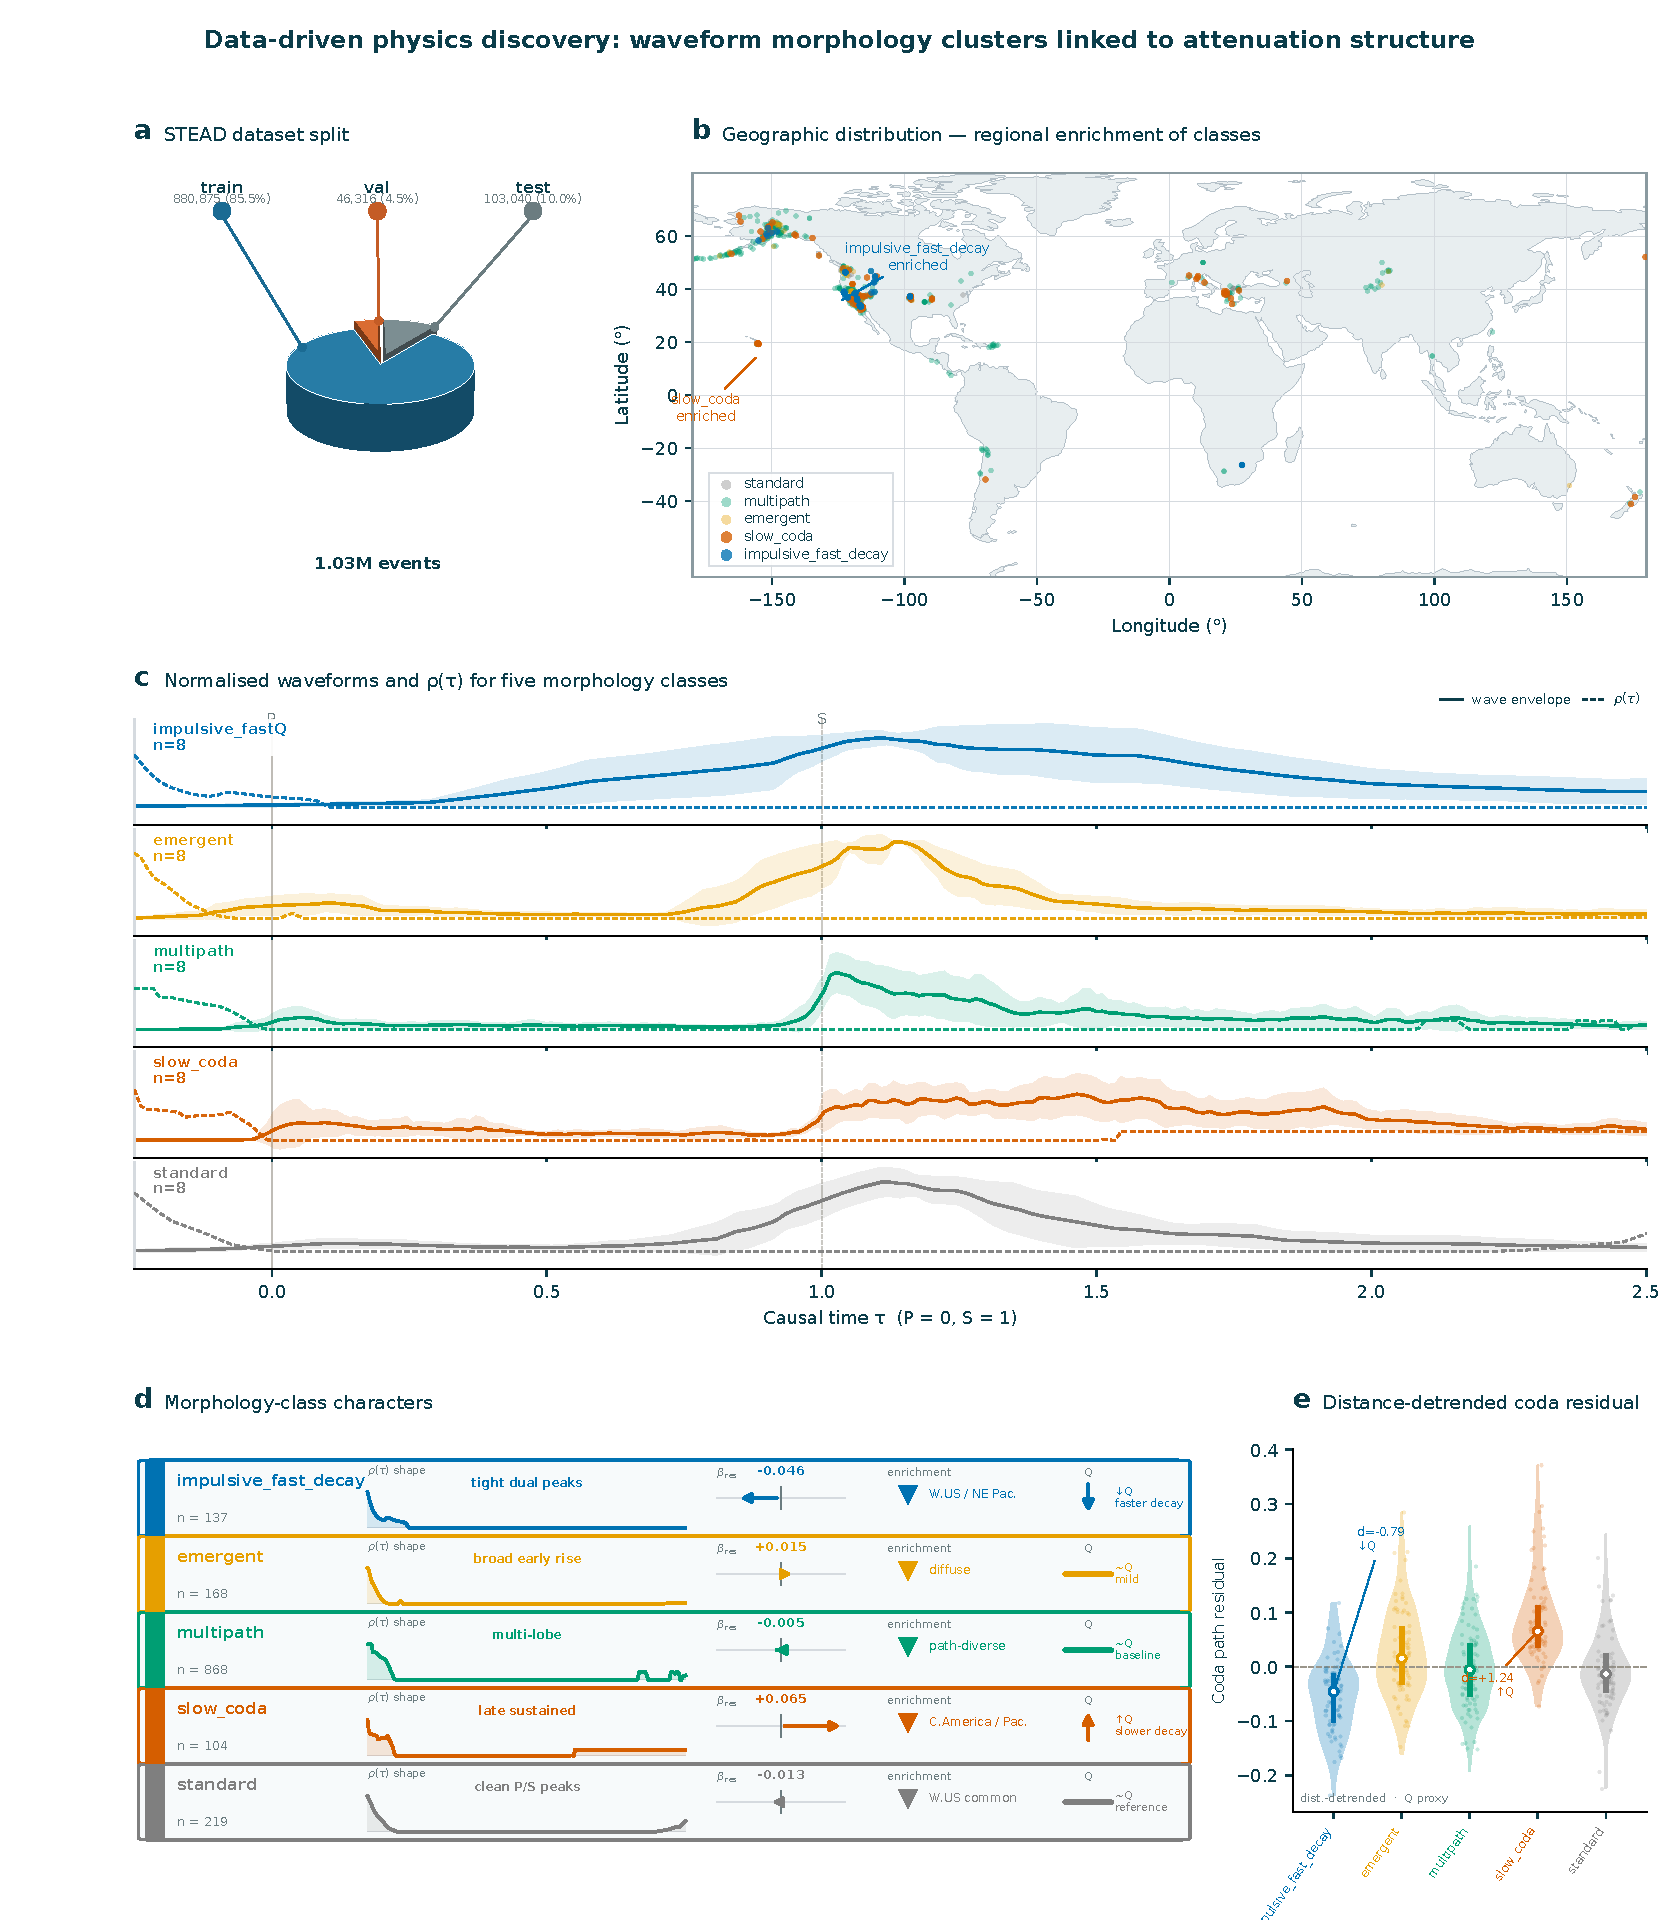
\includegraphics[
        trim=10mm 0mm 0mm 20mm,
        clip,
        width=0.95\textwidth
    ]{fig11.pdf}
  \caption{\textbf{Data-driven physics discovery: waveform morphology facies linked to attenuation structure.}
  \textbf{a},~STEAD local-earthquake split (\(1.03\,\mathrm{M}\) event traces; noise excluded): train \(880{,}875\) (\(85.5\%\)), validation \(46{,}316\) (\(4.5\%\)), test \(103{,}040\) (\(10.0\%\)).
  \textbf{b},~Geographic distribution of five frozen ceiling facies (not \(k\)-means labels). \(\mathrm{impulsive\_fast\_decay}\) is enriched in the western United States / northeast Pacific; \(\mathrm{slow\_coda}\) in Central America / Pacific. Marker size and opacity emphasise the two end-member classes.
  \textbf{c},~Class-mean normalised envelopes (solid) and delay-time densities \(\rho(\tau)\) (dashed) on causal time \(\tau\), with \(P=0\) and \(S=1\). Shading shows trace-to-trace spread (\(n=8\) examples per class). \(\mathrm{impulsive\_fast\_decay}\): sharp onset and short coda; \(\mathrm{emergent}\): gradual onset; \(\mathrm{multipath}\): multi-lobe \(\rho(\tau)\); \(\mathrm{slow\_coda}\): late sustained energy; \(\mathrm{standard}\): clean \(P\)/\(S\) peaks.
  \textbf{d},~Class characters: \(\rho(\tau)\) shape, median distance-detrended coda residual \(\beta_{\mathrm{res}}\), regional enrichment, and a \emph{post hoc} \(Q\) reading (\(\downarrow Q\), faster decay; \(\uparrow Q\), slower decay). Class names deliberately avoid presupposing \(Q\).
  \textbf{e},~Violin plots of \(\beta_{\mathrm{res}}\) by class (white marker: median; bar: interquartile range). Because coda slope enters the facies ceilings, panel~e is a \emph{characterization} of the taxonomy rather than an independent physical discovery: \(\mathrm{impulsive\_fast\_decay}\) is shifted negative (faster coda decay / lower apparent \(Q\)); \(\mathrm{slow\_coda}\) is shifted positive (slower decay / higher apparent \(Q\)). Annotated \(d\) values are Cohen's \(d\) versus all other classes. Independent evidence is deferred to geography and structure tests (Fig.~\ref{fig:main_single}).}
  \label{fig:shape-geo-coda}
\end{figure*}


\noindent

% =============================================================================
% INTRODUCTION
% =============================================================================
\section*{Introduction}

Scientific machine learning faces a methodological fork. Purely data-driven networks can achieve strong predictive scores, yet their representations rarely obey known causal physics and are difficult to trust as instruments of discovery. Physics-informed neural networks (PINNs)\cite{raissi2019pinn,karniadakis2021} improve consistency by adding PDE residuals as soft penalties, but physical adherence remains approximate, optimizable against data fit, and often post hoc in interpretation\cite{doumèche2025convergence}. A third family---partially interpretable hybrids---attaches saliency, probes, or symbolic heads to otherwise opaque backbones; the ``explanation'' is then correlative rather than constitutive of the computation\cite{vinuesa2023,ilievski2025}.

We take a stricter stance. \textbf{The primary contribution of this work is a differentiable physical probe}: known causal Green's functions are hard-wired as architectural primitives so that learning is confined to a small set of physically meaningful parameters. The model does not rediscover wave, diffusion, or Boltzmann memory laws from scratch; it \emph{uses} those laws to interrogate measurements. The resulting latents (\(\rho(t)\), kernel parameters, mode amplitudes) are readable because they inherit semantics from the probe, not because an external explainer is applied after training. This differs from both black-box predictors and soft physics-informed regularizers, and from differentiable simulators optimized for control\cite{hu2020difftaichi,xiao2025}: here the goal is discovery under known physics, not only prediction or actuation.

The shared primitive is the causal integral transform
\[
u(t)=\int_{0}^{t}\kappa(t-\tau)\,s(\tau)\,d\tau,
\]
the linear response that appears throughout wave propagation, diffusion, and viscoelastic memory\cite{akei2002,morse1953}. We instantiate three domain kernels with fixed functional form and learnable physical parameters (Fig.~\ref{fig:pnf-principle}d):
\begin{enumerate}
\item \textbf{Wave kernel} \(K_w(r)=\frac{1}{r+\varepsilon}e^{-\gamma r^{2}}e^{i\omega r}\) (with causal/light-cone support controlled by a learnable support parameter \(c\)), probing seismic waveforms for propagation structure.
\item \textbf{Diffusion kernel} \(K_d(r,t)=\frac{1}{(4\pi Dt)^{d/2}}e^{-r^{2}/(4Dt)}\), probing EEG montages for medium-like spatial responses.
\item \textbf{Memory kernel} \(K_m(t)=\sum_k G_ke^{-t/\lambda_k}\) (Prony/Maxwell), probing rheological spectra for readable relaxation masses.
\end{enumerate}
Kernel shapes are derived from known physics; Softplus-constrained parameters (\(\gamma,\omega,D,\lambda_k,\ldots\)) remain trainable. We call the architecture Physical Neural Field (\pnf{}).

A practical corollary of this strong inductive bias is \textbf{sample efficiency on scientific datasets}. Large catalogues such as STEAD allow competitive benchmarking, but many discovery settings---clinical EEG cohorts, paired rheology--chromatography melts---are small\cite{tripanpitak2026,dekeulenaer2025}. Because capacity is not spent relearning causal Green's functions, the same probe can still extract usable structure when \(n\) is modest\cite{sharma2025,lu2025}. Domains~II--III are therefore not side applications; they are stress tests of interpretability under data scarcity.

We evaluate three complementary claims, always following the frozen figure and table evidence: (I)~on STEAD, \pnf{} is competitive with EQTransformer and PhaseNet on most metrics while remaining physically structured, with explicit lags on selected scores; (II)~a diffusion leftover orthogonal to classical EEG voltmeter features associates with held-out cognition under neurodegeneration on AHEPA and is null on healthy-lifespan LEMON; (III)~memory-kernel mode masses align with GPC molecular-weight distributions far above a within-sample shuffle null. Across domains, fixed Green's-function probes supply readable latents; domain-specific discovery claims are the downstream readings.

Figure~\ref{fig:pnf-principle} lays out the complete logic of the PNF framework, using seismic picking as the running example. The starting point is a causal constraint: because seismic waveforms are time-series signals, any physically meaningful interaction between past and present must respect causality and finite propagation speed. This is encoded directly in the Huygens–Fresnel kernel (Fig.~\ref{fig:pnf-principle}a)—a fixed Green's-function form whose \(\gamma\), \(\omega\), and \(c\) are physics-indexed parameters governing locality, oscillation, and causal support scale (not claimed here as an identified medium velocity). With this kernel as the probe, the architecture (Fig.~\ref{fig:pnf-principle}b) embeds three-component waveforms, modulates them with a learned density \(\rho(t)\), and passes them through propagation blocks with fine and coarse branches to produce detection and P/S pick probabilities. The internal states already carry physical meaning (Fig.~\ref{fig:pnf-principle}c): \(\rho(t)\) rises at the P arrival and peaks during the S window, and the kernel amplitude concentrates its causal support just before onset—these are not post-hoc explanations but the computation itself. Finally, the same causal logic extends across domains (Fig.~\ref{fig:pnf-principle}d): the shared operator \(\mathcal{K}_\theta\) is instantiated as wave, diffusion, and memory kernels, each followed by domain-specific probe readings and discovery heads. The pattern is consistent: \emph{learn} \(\theta\), \emph{probe} phase-conditioned latents, and \emph{discover} structure that the known law does not explain. Anisotropic extensions replace scalar parameters by SPD tensors via Cholesky decomposition, following a unified principle detailed in Methods. The figure thus illustrates not merely an architecture, but a complete discovery workflow: first-principles physics defines the computation, and the readout exposes what the known law alone does not explain.

% =============================================================================
% RESULTS
% ============================================================================

\section*{Results}

\subsection*{A unified computational primitive for physical dynamics}

The causal integral transform defines the core primitive,
\[
\mathcal{T}[\kappa, s](t)=\int_{0}^{t}\kappa(t-\tau)\,s(\tau)\,d\tau,
\]
implemented in discrete form as a differentiable matrix--vector map \(v=Ku\). Wave, diffusion, and memory kernels share causal support but differ in Green's-function shape (Fig.~\ref{fig:pnf-principle}d). Parameters are Softplus-constrained and trained by gradient descent; the functional forms are not free neural approximations of the governing physics.

\subsection*{Domain I: Seismic phase picking and subsurface structure}

We evaluate \pnf{} on STEAD\cite{stead2019} under the standard \(0.5\,\mathrm{s}\) tolerance protocol\cite{mousavi2020eqt}. Table~\ref{tab:stead} compares full test-set detection and picking against EQTransformer\cite{mousavi2020eqt} and PhaseNet\cite{zhu2018phasenet}.

\paragraph{Competitive picking with an explicit accuracy--interpretability balance.}
With \(192\mathrm{k}\) parameters (about half of EQTransformer), \pnf{} matches EQTransformer on detection F1 (\(0.9989\)), improves S-wave F1 (\(0.9770\) vs.\ \(0.9731\) / \(0.9618\)), and achieves the lowest P-wave MAE (\(0.0169\,\mathrm{s}\) on the discrete \(800\)-bin/\(60\,\mathrm{s}\) grid; Methods). It does not dominate every cell: P-wave F1 (\(0.9852\)) trails EQTransformer (\(0.9897\)), and S-wave MAE (\(0.0878\,\mathrm{s}\)) trails PhaseNet (\(0.0801\,\mathrm{s}\)). Meanwhile, the Precision/Recall breakdown in Table~\ref{tab:stead} reveals a consistent pattern: PNF maintains strong recall across all heads (P-wave R \(0.9763\), S-wave R \(0.9643\)), indicating that the physics-constrained architecture reliably identifies genuine arrivals when they exist. The gap to EQTransformer is driven primarily by Precision (PNF P-wave P \(0.9942\) vs EQT \(0.9993\); S-wave P \(0.9900\) vs EQT \(0.9994\)), suggesting that the unconstrained transformer better suppresses false positives at the cost of a physically unreadable representation. We treat these differences as informative rather than disqualifying. A hard-wired Huygens--Fresnel kernel restricts the hypothesis class relative to unconstrained convolutional/attentive pickers; the model trades a fraction of peak picking score for readable latents that enable the structural discoveries below.

\paragraph{Frozen waveform facies from probe latents---not post-hoc clusters.}
Internal states carry predefined physics-indexed semantics (Fig.~\ref{fig:pnf-principle}c). From a frozen model checkpoint we export causal-chain observables---coda slope, onset sharpness, and multi-lobe structure in delay-time density \(\rho(\tau)\)---and assign each local-earthquake waveform to one of five facies using ceilings fixed \emph{before} any regional map was inspected: \textit{impulsive\_fast\_decay}, \textit{emergent}, \textit{multipath}, \textit{slow\_coda}, and \textit{standard}. These are not \(k\)-means labels. (Repository analysis tables retain the historical key \texttt{impulsive\_fastQ} for the same ceiling rule; the manuscript name drops the \(Q\) presupposition.)

The ceilings were chosen on the validation set to maximize separation in the three observables while preserving interpretability, and frozen before any test-set or spatial analysis was performed: peak-count threshold \(1.0\) distinguishes single-peaked from multi-peaked \(\rho(\tau)\); coda-fast/slow bounds \(-0.198\) and \(-0.113\) separate fast, intermediate, and slow decay on a log-linear scale; onset-high/low thresholds \(0.877\) and \(0.733\) capture the sharpness of the first arrival. Because coda slope participates in the ceilings, within-class coda contrasts (Fig.~\ref{fig:shape-geo-coda}e) are \emph{facies characterization}, not independent physical validation.

The data basis for this analysis is the test split of the STEAD local-earthquake catalogue, comprising over \(100{,}000\) traces after noise exclusion (Fig.~\ref{fig:shape-geo-coda}a). Mapping the geographic distribution of the five facies (Fig.~\ref{fig:shape-geo-coda}b)---a quantity that did not enter the ceilings---reveals a striking pattern: \textit{impulsive\_fast\_decay}---characterized by sharp onsets and rapid decay---is systematically enriched in the western United States and the northeast Pacific, whereas \textit{slow\_coda}---marked by prolonged tails and sustained energy---concentrates in Central America and the western Pacific. The association is not accidental; Cram\'er's \(V\approx0.37\) (FDR-adjusted \(p<0.001\)) indicates a moderate-to-strong relationship between facies identity and geographic region, even before any structural model is invoked. What distinguishes these classes morphologically becomes clear when their waveforms are resampled into a causal reference frame with P arrival at \(\tau=0\) and S arrival at \(\tau=1\) (Fig.~\ref{fig:shape-geo-coda}c). The class-mean normalized envelopes and \(\rho(\tau)\) profiles separate cleanly: \textit{impulsive\_fast\_decay} combines a sharp onset with a short coda; \textit{emergent} rises gradually with a broad peak; \textit{multipath} exhibits multiple lobes in \(\rho(\tau)\), indicating secondary arrivals; \textit{slow\_coda} sustains energy well past the S arrival; and \textit{standard} sits between these extremes with clean P and S peaks. The descriptive signatures of each class are summarized in Fig.~\ref{fig:shape-geo-coda}d--e. The probe therefore yields an interpretable taxonomy of coda shape rather than an opaque embedding cluster; geography and structure leftovers below provide the independent tests\cite{aki1969,aki1975,herraiz2023}.

\paragraph{Path-midpoint leftovers beyond distance, station, \(V_S\), and \(Q_S\).}
Having established that the probe yields interpretable facies, we now ask whether these facies carry information beyond what classical velocity and attenuation models already capture. Figure~\ref{fig:main_single} converts the same observables into a structure-controlled leftover. Coda slope is first distance-detrended to \(\beta\) against \(\log_{10}(\mathrm{dist}+1)\). A ridge expectation (\(\lambda=8\)) then removes \(\log_{10}\) distance, depth, magnitude, log-distance to nearest Quaternary fault, and station fixed effects; the residual \(\beta_{\mathrm{res}}\) is mapped at geographic path midpoints. In southern California (fixed stations; path distances \(20\)--\(120\,\mathrm{km}\)), two cells illustrate opposite path behaviour under same-station controls: Salton--Imperial midpoints decay faster than the same stations' other paths (site-median \(\Delta\beta\approx-0.032\); \(20\) stations), whereas eastern Transverse Ranges midpoints ring longer (\(\Delta\beta\approx+0.025\); \(15\) stations) (Fig.~\ref{fig:main_single}b,f,h).

The critical question is whether this leftover is already explained by existing observables. Three independence checks (Fig.~\ref{fig:main_single}c--e) rule out the most obvious alternatives. First, \(\beta_{\mathrm{res}}\) correlates with classical single-trace coda slope \(q_c\) (\(r=0.64\)), confirming that part of the leftover is conventional coda decay. Yet residualising on \(q_c\) still leaves coherent cell anomalies, and multipath versus slow-coda facies continue to separate inside matched \(q_c\) terciles—indicating that the leftover is not simply a proxy for standard coda slope. Second, sampling Berg et al.\ upper-crust \(V_S\) at path midpoints yields near-null correlation (\(r=-0.08\)); the Salton and Transverse Ranges cells occupy the same \(V_S\) band yet opposite \(\beta_{\mathrm{res}}\)\cite{berg2021}. If the leftover were just a velocity effect, it could not split two regions with indistinguishable \(V_S\). Third, Lin \& Jordan direct-wave \(Q_S\) is likewise nearly orthogonal (\(r=-0.07\)); removing \(Q_S\) leaves cell \(\Delta\beta\) essentially intact, and the Salton cell can combine relatively high direct-wave \(Q_S\) with faster coda decay\cite{lin2023}. This is the intended scientific reading: coda-path leftovers retain information \emph{not captured by the examined linear summaries} of published upper-crust \(V_S\) and direct-wave \(Q_S\) at path midpoints---not a claim of complete physical independence from all velocity or attenuation structure. Near-null Pearson correlations can also arise from resolution mismatch, kernel differences, midpoint approximation, measurement noise, or coda versus direct-wave sensitivity\cite{lin2023,delpezzo2023,prudencio2022}. Same-station controls reduce site effects but do not fully remove source--path coupling (focal mechanism and event clustering are not modelled as fixed effects here).


\begin{figure*}[!t]
  \centering
  
\includegraphics[trim=0mm 0mm 0mm 10mm,
    clip=true, width=\textwidth]{Fig_main_single.pdf}
  \caption{\textbf{From waveform facies to a structure-controlled path residual.}
  \textbf{(a)}~Pipeline: local earthquake waveforms yield frozen, interpretable
  observables and five facies; coda slope is distance-detrended to $\beta$, then
  residualized against structure and station effects to give path-midpoint
  leftover $\beta_{\mathrm{res}}$. Absorbing ($\beta_{\mathrm{res}}{<}0$) versus
  ringing ($\beta_{\mathrm{res}}{>}0$) envelopes, and the same-station control
  geometry, are shown schematically.
  \textbf{(b)}~Same-station median $\Delta\beta$ for SoCal and Cascadia sites
  (negative = absorbing, positive = ringing).
  \textbf{(c--e)}~Independence checks: $\beta_{\mathrm{res}}$ versus classical
  coda-decay slope $q_c$ ($r{=}0.64$), Berg et al.\ (2021) path-mid $V_S$
  ($r{=}{-}0.08$), and Lin et al.\ (2023) path-mid $Q_S$ ($r{=}{-}0.07$);
  highlighted cells \#2 (Salton) and \#5 (ETR).
  \textbf{(f)}~SoCal map of path-midpoint $\beta_{\mathrm{res}}$.
  \textbf{(g)}~Out-of-region Cascadia replica with the same color scale.
  \textbf{(h)}~Synthesis of absorbing versus ringing domains and leftover cell
  $\Delta\beta$ after removing $q_c$, $V_S$, or $Q_S$, with a Salton-path
  prediction.
  }
  \label{fig:main_single}
\end{figure*}

\begin{figure*}[!t]
  \centering
  
\includegraphics[trim=0mm 0mm 0mm 10mm,
    clip=true, width=\textwidth]{eeg_impact_discovery.pdf}
  \caption{\textbf{Voltmeter-orthogonal EEG probe leftover associates with held-out cognition under neurodegeneration.}
  \textbf{(a)}~Cohort composition for the clinical AHEPA set ($n{=}88$; HC/FTD/AD)
  and the healthy-lifespan LEMON set ($n{=}202$; young/old).
  \textbf{(b)}~Analysis pipeline: eyes-closed 19-channel EEG is summarized by a
  classical voltmeter (age, sex, $\theta/\alpha$, band-power $\alpha$) and a frozen
  spatial probe yielding a diffusion-probe index $D_{\mathrm{eff}}=1/\rho_{\mathrm{std}}$ (numerical floor) and $\rho(t)$. A train-only residualizer
  defines
  $\mathrm{leftover}=D_{\mathrm{eff}}-f_{\mathrm{train}}(\mathrm{volt})$,
  applied out of sample without refit. Controls: diffusion Green kernel (phase off),
  oscillatory phase on the kernel (physics kill), and agreement of two spatial kernels.
  \textbf{(c)}~Held-out case epochs (HC, FTD, AD): stacked 10--20 channels,
  medium density $\rho(t)$, scalp RMS topography, and band-power share.
  \textbf{(d)}~Held-out association between train-fit leftover and
  MMSE residualized on the voltmeter with the same train-only fit
  (Spearman $\rho{=}{-}0.24$, $n{=}31$; Pearson $r{=}{-}0.30$).
  Complementary LOSO / capacity-matched nulls are reported in Methods.
  \textbf{(e)}~Probe-physics control: in-split MMSE $\Delta R^{2}$ relative to the
  voltmeter is largest for the Fresnel probe, reduced for anisotropic diffusion with
  phase off, and near zero with phase on.
  \textbf{(f)}~Fresnel and anisotropic leftovers collapse onto one axis on held-out
  subjects (Spearman $\rho{=}0.92$, $p{=}1{\times}10^{-13}$, $n{=}31$).
  \textbf{(g)}~Discovery summary: leftover tracks cognition under neurodegeneration
  (AHEPA, $|\rho|$ vs.\ MMSE$|\,\mathrm{demo}$), but is null against healthy aging,
  GM/ICV, and TMT on LEMON.
  }
  \label{fig:eeg_impact_discovery}
\end{figure*}


\paragraph{Out-of-region replication and a falsifiable prediction.}
Do these SoCal-specific findings generalize, or are they artefacts of a particular tectonic setting? The identical frozen ceilings and residualization pipeline applied to Cascadia STEAD paths recovers a Salton-signed faster-decay residual near Mount St.~Helens and a ringing residual near Seattle (Fig.~\ref{fig:main_single}g). The sign agreement—without refitting any facies rules—is an out-of-region replica that substantially reduces the chance of overfitting to SoCal geology. Source-bin / magnitude / year jackknives on the SoCal Salton and eastern Transverse Ranges cells themselves remain sign-stable (STABLE; \(\ge80\%\) of qualifying tests keep the expected \(\Delta\beta\) sign with \(p<0.05\) and \(n_{\mathrm{sites}}\ge8\); Methods). A pre-registered style prediction follows from the SoCal cells: if the Salton cell reflects a genuine absorption feature, new paths whose midpoints fall there should show same-station \(\Delta\beta\le-0.02\) once \(\ge8\) stations are available; the Seattle cell, representing the opposite regime, predicts the opposite inequality. This prediction is not a post-hoc curve fit; it is a direct consequence of the probe's reading that coda attenuation carries path information not captured by the examined linear summaries of published \(V_S\) and \(Q_S\) models. Joint out-of-sample residualisation confirms the same point quantitatively: five-fold OOS \(R^{2}\) of \(\beta_{\mathrm{res}}\) explained by Berg \(V_S\), Lin \(Q_S\), or their linear/quadratic combination remains \(\lesssim0.01\) (Methods).


\paragraph{Velocity inversion via Physics Decoder.}
The preceding analyses established that the probe latents carry physically meaningful structure—facies and path residuals relative to the examined classical summaries. This raises a natural question: can the same latents also be read out for a different physical task? To test this, we attach a lightweight Physics Decoder (a 2-layer MLP on frozen \pnf{} latents) that maps probe features—\(\rho(t)\), envelope statistics, kernel parameters, and pick probabilities—to layered \((v_P,v_S)\) models, initialising differentiable FWI (Fig.~\ref{fig:pnf-principle}d, bottom)\cite{tarantola1984,virieux2009,huang2023}. On the reported protocol, \(69.6\%\) of real STEAD events (\(n=500\), Wilcoxon \(p<0.001\)) improve convergence relative to perturbed baselines, with mean travel-time misfit reduced from \(11.22\) to \(3.08\). This supports transferability of probe latents beyond picking: the same internal states that organise waveform facies and path residuals also carry information usable for layered velocity initialisation. The Physics Decoder remains an initialisation aid rather than an oracle travel-time solver, and should not be read as a claim of fully recovered subsurface structure.


\subsection*{Domain II: A physical probe for EEG medium leftovers under neurodegeneration}

Domain~II tests whether the \emph{same} causal primitive, instantiated as a spatial diffusion/Fresnel probe, can extract scientifically usable structure from modest clinical EEG (Fig.~\ref{fig:eeg_impact_discovery}). Unlike the seismic benchmark, where large labelled datasets enable direct performance comparison, EEG discovery settings are typically small. The design is therefore deliberately not a classifier leaderboard—it asks instead whether a train-only residualizer
\(\mathrm{leftover}=D_{\mathrm{eff}}-f_{\mathrm{train}}(\mathrm{volt})\)
isolates probe variance orthogonal to classical voltmeter features (age, sex, \(\theta/\alpha\), band-power \(\alpha\)), and whether that leftover is associated with neurodegeneration-context cognition\cite{timmers2022,sohrabpour2025}. Here \(D_{\mathrm{eff}}\) denotes a diffusion-\emph{probe index} (operationally \(1/\rho_{\mathrm{std}}\) with a numerical floor), not a claim that \(\rho(t)\) is a recovered tissue diffusivity.

\paragraph{Held-out association under neurodegeneration.}
On AHEPA held-out subjects, train-fit leftover associates with MMSE residualized on the voltmeter using the same train-only fit (Spearman \(\rho=-0.24\), \(n=31\); Fig.~\ref{fig:eeg_impact_discovery}d; Pearson \(r=-0.30\) on the same pool; test-only Pearson \(r=-0.37\), \(n=18\))\cite{jeong2004}. Leave-one-held-out-subject intervals keep the Spearman median near \(-0.25\) (bootstrap 95\% CI on the LOSO median \([-0.25,-0.23]\)). Train-shuffle and capacity-matched random-feature nulls yield mean \(|\rho|\approx0.05\)--\(0.07\) with \(p_{\ge\mathrm{obs}}\approx0.002\) (Methods). Case epochs illustrate readable \(\rho(t)\) and topography alongside band summaries (Fig.~\ref{fig:eeg_impact_discovery}c). This provides preliminary held-out evidence that a train-only residualizer can isolate probe variance orthogonal to the classical voltmeter features, with the association exceeding matched-capacity nulls even when the pooled Spearman point estimate is modest.

\paragraph{Mechanism and construct controls.}
Following Fig.~\ref{fig:eeg_impact_discovery}e, in-split MMSE \(\Delta R^{2}\) relative to the voltmeter is largest for the Fresnel probe, reduced for anisotropic diffusion with phase off, and near zero when oscillatory phase is added to the Green kernel (physics kill). Fresnel and anisotropic leftovers collapse onto one held-out axis (Spearman \(\rho=0.92\), \(p=1\times10^{-13}\), \(n=31\); Fig.~\ref{fig:eeg_impact_discovery}f). These controls are essential: they rule out the possibility that the leftover is a generic artefact of any differentiable kernel\cite{vinuesa2023,sharma2025}. The association was sensitive to the chosen kernel structure; when oscillatory phase is added, the in-split gain collapses.

\paragraph{Healthy-lifespan negative control.}
On independent LEMON adults (\(n=202\)), the leftover is null against healthy aging, GM/ICV, and TMT (Fig.~\ref{fig:eeg_impact_discovery}g). This is an independent-dataset negative-control analysis, not a second clinical replication: it is consistent with disease-context specificity but does not by itself prove pathology specificity. Absolute probe scale remains domain-shifted across cohorts and is treated as a methods constraint, not a transportable clinical index without calibration.

Together, Domains~I--II illustrate the intended contribution: a physically grounded probe can isolate voltmeter-orthogonal variance associated with held-out cognition in a modest neurodegenerative EEG cohort, with a null pattern against the examined healthy-lifespan endpoints. This supports the broader claim that known physics, when used as a probe, can yield domain-relevant structure even when labelled cohorts are modest.

\begin{figure*}[!t]
  \centering
  
\includegraphics[trim=0mm 0mm 0mm 15mm,
    clip=true, width=\textwidth]{rheo_impact_discovery.pdf}
  \caption{\textbf{Readable PNF mode masses align with GPC MWD above a shuffle null.}
  \textbf{(a)}~Cohorts: Leeds paired SAOS$\cap$GPC melts ($n{=}9$; linear vs.\ branched)
  and roles of paired versus external probes (UMN SAOS, PolyWeight OOD);
  only paired samples enter the discovery test.
  \textbf{(b)}~Pipeline: SAOS master curves $\rightarrow$
  \textbf{PNF} (fixed-$\tau$ library $\rightarrow G_k$) $\rightarrow$
  tube map $M\propto\lambda^{1/\alpha}$ aligning mode mass with GPC $\rightarrow$
  discovery test of
  $\mathrm{corr}(G_k/\sum G,\,\mathrm{GPC\ mass})$
  against a within-sample shuffle-$G_k$ null;
  controls include $\alpha$/free-$\lambda$ robustness and Elliott NN
  (\emph{for compare}).
  \textbf{(c)}~Key cases (PS3, PS1, A1PS): measured $G'$, $G''$ with PNF
  reconstruction and topology insets; corresponding GPC $w(M)$ with
  per-sample tube $r$, null mean, and significance.
  \textbf{(d)}~Per-sample tube correlation: observed $\gg$ shuffle null
  (mean $r{=}0.911$ vs.\ $0.565$; $\Delta{=}0.35$; $89\%$ of samples $p{<}0.05$).
  \textbf{(e)}~Robustness across tube exponent $\alpha\in\{3.0,3.4,3.7\}$,
  free-$\lambda$, and SAOS-bin proxy; absolute $r$ is partly structural,
  so $\Delta$ versus null is the primary evidence.}
  \label{fig:rheo-impact-discovery}
\end{figure*}

\subsection*{Domain III: Molecular alignment from rheological spectra}

Domain~III pushes the same thesis to its extreme: if the probe can read physically meaningful structure from just nine paired samples, this provides a preliminary stress test in a small-data regime. The test case is Leeds polystyrene SAOS$\cap$GPC melts ($n=9$), with external SAOS-only and OOD roles shown in Fig.~\ref{fig:rheo-impact-discovery}a but excluded from the discovery test. The memory kernel is identified as a fixed-$\tau$ Prony/Maxwell library (PNF) on SAOS master curves. The question is whether the learned mode masses $G_k/\sum G$ align with GPC-measured molecular weight distribution under the tube-theory mapping $M\propto\lambda^{1/\alpha}$\cite{doi1986,degennes1971,rubinstein1987,winey2019}---a physically grounded relationship between relaxation time and molecular mass. The alignment is tested against a within-sample shuffle-$G_k$ null (Fig.~\ref{fig:rheo-impact-discovery}b).

\paragraph{Readable amplitudes align with MWD above shuffle null.}
Key cases---PS3 (linear), PS1 (linear but structurally challenging), and A1PS (branched)---illustrate the range of outcomes (Fig.~\ref{fig:rheo-impact-discovery}c). PS3 shows clean SAOS reconstruction and strong alignment; PS1 achieves high observed \(r\) but also high shuffle null, resulting in a small \(\Delta\); A1PS, a branched melt, deviates from the linear tube-theory scaling, consistent with the known physics of branched polymer relaxation. Across all samples, observed tube correlations (mean \(r=0.911\)) exceed the shuffle null (mean \(r=0.565\); \(\Delta=0.35\); 8 out of 9 samples \(p<0.05\); Fig.~\ref{fig:rheo-impact-discovery}d). Under the same fixed-\(\lambda\) library, PNF spectrum fits match classical Prony NLS on Leeds SAOS (mean rel-log \(0.0326\) for both), so the discovery claim rests on the tube--MWD reading and shuffle null rather than on a novel optimiser. Synthetic recovery further shows that mode masses are identifiable under that library (mean mass Spearman \(0.86\); Methods). Robustness holds across \(\alpha\in\{3.0,3.4,3.7\}\), free-\(\lambda\), and a SAOS-bin proxy (Fig.~\ref{fig:rheo-impact-discovery}e). As emphasised in the figure, absolute \(r\) is partly structural; \textbf{\(\Delta\) versus null is the primary evidence}.

The one non-significant sample (PS1) reinforces this reading in another way. Its observed tube \(r\approx0.96\) is high, but the shuffle null is also high (\(r\approx0.88\)), so \(\Delta\approx0.08\) is small. This confirms that absolute \(r\) alone would overstate the evidence, and that \(\Delta\) versus null is the correct metric---exactly as emphasised in Fig.~\ref{fig:rheo-impact-discovery}e. PSA and PS8, by contrast, show large \(\Delta\) and clear significance. The distinction is not whether the alignment exists, but whether it exceeds random mass assignment. This pattern is consistent with independent observations: PS1 is also difficult for Elliott NN and LOO benchmarks, suggesting that the challenge lies in the sample's distribution geometry rather than a failure of the PNF probe.

This domain is one more demonstration of the probe's value in the small-data regime: with nine paired melts, the memory kernel yields a molecular alignment whose statistical significance is established through a within-sample shuffle null---a level of falsifiability that unconstrained spectral fitting, even when accurate, does not automatically provide. The Elliott NN ensemble, while included as a representative data-driven comparator, is not treated as a performance ceiling; rather, it underscores the distinction between black-box prediction and physically readable inference\cite{llm4sd2025,berner2026}. The key point is not that the probe outperforms black-box models on every metric---it is that the probe's output can be read and verified as physics, whereas the black-box output cannot.

\subsection*{Cross-domain synthesis}

Across domains, the evidence from the frozen analysis protocols supports one methodological pattern. (i)~Hard-wired causal kernels produce competitive large-data performance with an explicit metric trade-off (Table~\ref{tab:stead}). (ii)~Readable latents enable discovery pipelines---facies/path residuals, voltmeter-orthogonal leftovers, tube-aligned mode masses---rather than post-hoc attribution of opaque embeddings. (iii)~Small scientific cohorts (EEG, rheology) remain usable precisely because the probe encodes known physics. Validation styles differ by necessity: STEAD is benchmark comparison; EEG combines held-out association with a healthy negative control; rheology combines within-sample mechanistic nulls, parameter robustness, Prony-NLS equivalence, and synthetic mode-mass recovery. These are complementary pillars of scientific argument, not interchangeable substitutes for one another.

Together, they converge on a single conclusion: the same differentiable physical probe---instantiated as wave, diffusion, or memory kernel---can be read for domain-relevant structure when the same design principle is instantiated with domain-specific Green's-function probes, even when labels are scarce.


% =============================================================================
% DISCUSSION
% =============================================================================
\section*{Discussion}

\paragraph{Contribution: an interpretable differentiable physics probe.}
The central contribution is methodological. We propose that known causal Green's functions can serve as \emph{computational instruments}: fixed-form, differentiable probes whose parameters remain scientifically readable. This is distinct from black-box predictors, from PINNs that encode physics as soft, violable penalties\cite{raissi2019pinn,karniadakis2021}, and from post-hoc explanation of opaque embeddings\cite{ilievski2025,llm4sd2025}. Interpretability here is constitutive---the computation \emph{is} the probe---rather than decorative. The discussion proceeds through three lenses: what the probe reads (discovery), where it works best (small data), and what it costs (accuracy).

\paragraph{Physics as probe, not as constraint.}
When physics is only a constraint, success is a prediction that approximately obeys a law. When physics is a probe, success is a measurement of structure the law alone does not name. In seismology, wave-kernel latents organise morphology facies and path leftovers beyond the examined linear \(V_S\)/\(Q_S\) summaries (Figs.~\ref{fig:shape-geo-coda}--\ref{fig:main_single})\cite{aki1969,aki1975,lin2023}. In EEG, diffusion/Fresnel leftovers isolate voltmeter-orthogonal variance that associates with held-out cognition under neurodegeneration yet is null against the examined healthy-lifespan endpoints (Fig.~\ref{fig:eeg_impact_discovery})\cite{tripanpitak2026,sohrabpour2025}. In rheology, Prony mode masses align with MWD above shuffle nulls (Fig.~\ref{fig:rheo-impact-discovery})\cite{doi1986,degennes1971}. In each case a fixed Green's function supplies the computational probe; the specimen is the data; the reading is the domain-specific discovery claim.

The discoveries themselves are threefold. In seismology, the probe indicates that coda-path leftovers retain information not absorbed by the examined published upper-crust \(V_S\) and direct-wave \(Q_S\) midpoint summaries---a pattern replicated in a second tectonic setting and codified as a falsifiable prediction\cite{lin2023,delpezzo2023,herraiz2023}. In EEG, a diffusion-derived leftover emerges as a candidate cognition-associated signal in a neurodegenerative cohort and is null against the examined healthy-lifespan endpoints\cite{jeong2004,sohrabpour2025,casas2025}. In rheology, learned mode masses align with independently measured molecular-weight distributions above shuffle nulls in nine paired melts\cite{doi1986,elliott2025,winey2019}. These are three independent readings from the same design principle, each falsifiable in its own domain.

\paragraph{Small-data regimes as a design target.}
Domains~II--III are intentionally small. This is not a limitation to be excused but a design choice that tests the probe where it matters most: when paired labels are scarce, a purely data-driven model would have little to learn from, yet the physics-constrained probe still yields falsifiable structure. Their value is not that they replace large-scale clinical or materials programmes, but that a strong physical prior can keep discovery feasible when \(n\) is modest\cite{zhai2025,lu2025,sharma2025}. Sample efficiency is therefore an advantage of the probe design; small sample sizes do not by themselves establish definitive domain-level validation.

\paragraph{The cost of a strong prior: accuracy--interpretability balance.}
Table~\ref{tab:stead} makes the trade-off quantitative. \pnf{} wins or ties on several STEAD metrics with fewer parameters, yet trails EQTransformer on P-wave F1 and PhaseNet on S-wave MAE. We interpret these gaps as the price of restricting the hypothesis class to causal wave kernels with readable parameters. For settings where mechanistic auditability matters---hazard assessment, clinical EEG, materials identification---that exchange can be favourable; for pure leaderboard picking it may not be. The paper's thesis is not that interpretability dominates all metrics, but that it should be reported as an explicit scientific trade-off.

\paragraph{From physics-informed to physics-as-computation.}
The distinction is architectural. PINNs ask models to obey physics; PNF asks models to \emph{compute with} physics. Soft penalties can be traded away when they conflict with data fit; hard-wired kernels cannot without changing the instrument itself. This is the deeper claim: interpretability here is not an add-on but a constitutive property of the computation\cite{vinuesa2023,ilievski2025}. We envision a library of composable causal primitives for linear and eventually nonlinear regimes, always with readable parameters and domain-appropriate null controls\cite{berner2026,zhai2025}.

\paragraph{Limitations and outlook.}
Several limits are intrinsic to the present evidence. Seismic processing remains tied to fixed temporal grids; the Physics Decoder aids FWI initialisation but does not match oracle travel-time solvers. Cascadia replicates the residualization pipeline but lacks Berg/Lin cubes for the same independence battery applied in SoCal; SoCal source-bin jackknives and joint \(V_S\)+\(Q_S\) OOS \(R^{2}\) now harden the leftover claim, while focal-mechanism catalogues remain unavailable in the STEAD export used here. EEG associations use modest held-out \(n=31\); under a consistent train-fit protocol the pooled Spearman is modest (\(\rho=-0.24\)), with stronger test-only Pearson and LOSO/null hardening reported in Methods---predictive \(\Delta R^{2}\) should still not be overstated. LEMON is a negative control, not a second AD/FTD replication site. Rheology rests on \(n=9\) paired melts; absolute tube \(r\) is partly structural (SAOS-bin proxy). Synthetic recovery now covers Prony masses, wave \((\gamma,\omega)\) (with weak \(c\)), and EEG diffusion anisotropy; full profile-likelihood audits and additional tectonic/clinical cohorts remain open. These are not failures but honest boundaries of the current evidence. The same logic that made the probe work here---fixed Green's functions, readable parameters, domain-appropriate nulls---can be extended to full 2-D/3-D inversion, to nonlinear kernels, and to other wave-like systems\cite{huang2023,xiao2025}. The paradigm is not tied to seismology, EEG, or rheology; it is tied to the availability of a causal Green's function and a question worth asking.

% =============================================================================
% METHODS
% =============================================================================

\section*{Methods}

\subsection*{Causal integral transform as a computational primitive}

The shared operator is the causal convolution
\begin{equation}
u(t)=\int_{0}^{t}\kappa(t-\tau)\,s(\tau)\,d\tau,
\label{eq:causal}
\end{equation}
discretised as a differentiable map \(v=Ku\). Kernel \emph{shapes} are fixed Green's functions of known linear physics; a small set of physically meaningful parameters is Softplus-constrained and trained by gradient descent. This makes \pnf{} compute \emph{with} known causal physics rather than rediscovering it with an unconstrained network.

\subsection*{Wave kernel (seismic)}

The production seismic probe is a Huygens--Fresnel wave kernel with causal/light-cone support\cite{akei2002,morse1953},
\begin{equation}
K_w(r)\propto \frac{e^{-\gamma r^{2}}e^{i\omega r}}{r+\varepsilon}\,\chi(\theta)\,M(r),
\end{equation}
where \(r\) is temporal lag (equivalently a travel-time proxy), \(M(r)\) enforces \(r>0\) and finite speed, \(\gamma\) controls attenuation/locality, \(\omega\) sets oscillation, and \(\chi(\theta)=\tfrac12(1+\cos\theta)\) is an obliquity factor. Fine and coarse \(\omega\) branches specialise P- and S-sensitive pathways (Fig.~\ref{fig:pnf-principle}b). Anisotropic extensions replace scalar metrics by SPD direction-dependent distances \(r_{\mathrm{eff}}=\sqrt{\Delta\mathbf{x}^{\top}\mathbf{M}\Delta\mathbf{x}}\) with \(\mathbf{M}=\mathbf{L}\mathbf{L}^{\top}\).

\subsection*{Diffusion kernel (EEG)}

The EEG probe uses spatial diffusion / Fresnel Green's functions on the 10--20 montage\cite{lopes1997},
\begin{equation}
K_d(\mathbf{r},t)=\frac{1}{(4\pi t)^{d/2}\sqrt{\det\mathbf{D}}}
\exp\!\Big(-\frac{\mathbf{r}^{\top}\mathbf{D}^{-1}\mathbf{r}}{4t}\Big)H(t),
\end{equation}
with \(d=2\) and learnable SPD \(\mathbf{D}\). We report an effective scalar \(D_{\mathrm{eff}}=1/\rho_{\mathrm{std}}\) (clipped at \(10^{-6}\)) as the probe summary used by the residualizer. Oscillatory phase can be added to the Green kernel as a physics-kill control (``phase on''); the discovery board uses phase-off diffusion alongside a Fresnel spatial probe.

\subsection*{Memory kernel (rheology)}

Linear viscoelastic SAOS identification uses a Prony/Maxwell memory
\begin{equation}
K_m(t)=\sum_{k=1}^{K}G_ke^{-t/\lambda_k},
\end{equation}
with a fixed log-spaced \(\lambda\) library (\(K=8\)) matched to each sample's \(\omega\) band (PNF; same physics as classical Prony NLS)\cite{ferry1980}. Complex moduli follow
\(G'(\omega)=G_{\infty}+\sum_k G_k\frac{(\omega\lambda_k)^{2}}{1+(\omega\lambda_k)^{2}}\) and
\(G''(\omega)=\sum_k G_k\frac{\omega\lambda_k}{1+(\omega\lambda_k)^{2}}\).
Fits minimise log-modulus residuals. Free-\(\lambda\) fits and SAOS-bin proxies are reserved for robustness (Fig.~\ref{fig:rheo-impact-discovery}e). Tube-style maps use \(M\propto\lambda^{1/\alpha}\) with primary \(\alpha=3.4\)\cite{doi1986}. Anisotropic materials extend \(G_k\to\mathbf{W}_k=\mathbf{L}_k\mathbf{L}_k^{\top}\).


% Fig. layout.pdf - Overall PNF architecture data flow
\begin{figure}[t]
    \centering
    \includegraphics[width=\columnwidth]{layout.pdf}
    \caption{\textbf{Overall data flow of the PNF seismic architecture.}
    Three-component waveforms \(x \in \mathbb{R}^{B \times 800 \times 3}\) enter the source embedding layer, pass through the multi-scale Huygens propagation encoder, and are decoded into detection and P/S pick probabilities. The overall flow follows the five-stage design described in the main text.}
    \label{fig:layout}
\end{figure}

% Fig. encoder.pdf - Multi-scale wave propagation encoder
\begin{figure}[t]
    \centering
    \includegraphics[width=0.8\columnwidth]{encoder.pdf}
    \caption{\textbf{Multi-scale Huygens propagation encoder.}
    The embedded representation is processed through fine (downsample=1, causal window \(8\,\mathrm{s}\)) and coarse (downsample=2, causal window \(20\,\mathrm{s}\)) branches, each with three WaveBlock layers (production multi-scale encoder). After linear projections, the branches are concatenated, passed through a linear layer (\(256\to128\)), LayerNorm, and GELU, then split back into real and imaginary components \(h_r, h_i\).}
    \label{fig:encoder}
\end{figure}

% Fig. decoder.pdf - Physics Decoder for velocity inversion
\begin{figure}[t]
    \centering
    \includegraphics[width=0.9\columnwidth]{decoder.pdf}
    \caption{\textbf{Physics Decoder architecture.}
    The frozen backbone exports \(h_r, h_i\), \(\rho(t)\), kernel parameters \((\gamma,\omega,c)\), and picks. A feature extraction module computes waveform statistics and kernel summaries, then per-station to event-mean pooling. The Macro Physics Head (MLP: \(48\to48\to3\)) predicts scale, contrast, and \(V_S/V_P\) ratio, converted to layered \(v_P, v_S\) models. Geographic coordinates \((x,y)\) are optional inputs.}
    \label{fig:decoder}
\end{figure}

\subsection*{Network architecture}

The \pnf{} architecture for seismic waveform processing follows a five-stage design, with the overall data flow shown in Fig.~\ref{fig:layout}. The multi-scale propagation encoder (Fig.~\ref{fig:encoder}) implements the core Huygens wave-block processing, while the Physics Decoder (Fig.~\ref{fig:decoder}) attaches to the frozen backbone for downstream velocity inversion.

\textbf{(1) Source embedding.} Input three-component waveforms \(x \in \mathbb{R}^{B \times 800 \times 3}\) (batch \(\times\) time \(\times\) channel) are projected to a shared latent representation of width \(D=64\). The embedding layer maps each time sample independently, producing \(h_r, h_i \in \mathbb{R}^{B \times 800 \times 64}\), where the real and imaginary components separately initialise the in-phase and quadrature pathways of the subsequent wave propagation blocks.

\textbf{(2) Multi-scale wave propagation.} The embedded representation is processed through a Huygens propagation module with two parallel branches operating at different temporal resolutions (Fig.~\ref{fig:encoder}). In the production multi-scale encoder, the \textit{fine branch} (downsample factor 1) preserves full temporal resolution with a causal local window of \(8\,\mathrm{s}\); the \textit{coarse branch} (downsample factor 2) operates at half the temporal resolution with a wider window of \(20\,\mathrm{s}\) (derived from a base \(15\,\mathrm{s}\) local-window hyperparameter via \(\min(8,15)\) / \(\max(20,15)\)). Each branch contains three WaveBlock layers that apply the learned Huygens--Fresnel kernel with branch-specific kernel parameters \((\gamma,\omega,c)\). After propagation, the fine and coarse representations are independently passed through linear projections and then concatenated, followed by a linear layer (\(256 \to 128\)), LayerNorm, and GELU activation. The final representation is split back into real and imaginary components \(h_r, h_i \in \mathbb{R}^{B \times 800 \times 64}\), combining the coarse branch's long-range context with the fine branch's timing precision for subsequent task-specific decoding.

\textbf{(3) Medium density estimation.} A separate causal convolutional network estimates the medium density field \(\rho(t) \in \mathbb{R}^{B \times 800 \times 1}\), a Softplus-constrained latent variable that modulates the secondary-source amplitudes in subsequent kernel propagation. In the seismic domain, \(\rho(t)\) rises at P arrival and peaks during the S window; in EEG, \(\rho(t)\) encodes neural activity density.

\textbf{(4) Task branches with dedicated kernel parameters.} The wavefield representation and density field are passed through a final Huygens propagation block with task-specific kernel parameters. For seismic picking, fine and coarse \(\omega\) branches handle P- and S-sensitive pathways separately.

\textbf{(5) Output heads.} The propagated representation is decoded into task-specific outputs: detection logits and P/S pick probabilities for STEAD. For EEG applications, the same architecture is adapted with 19-channel input and clinical classification heads.

\textbf{Physics Decoder for velocity inversion.} A lightweight Physics Decoder attaches to the frozen backbone to extract probe features for downstream inversion (Fig.~\ref{fig:decoder}). The frozen backbone exports real and imaginary wavefield components \(h_r, h_i\), density \(\rho(t)\), kernel parameters \((\gamma,\omega,c)\), and pick probabilities. A feature extraction module computes waveform statistics and kernel summaries, then performs per-station to event-mean pooling. The Macro Physics Head---an MLP with dimensions \(48 \to 48 \to 3\)---predicts three macro parameters (scale, contrast, \(V_S/V_P\) ratio), which are then converted to layered \(v_P\) and \(v_S\) models (typically \(L=5\) layers) and optionally \(Q\). Geographic coordinates \((x,y)\) can be included as an optional input to account for regional variations.

\textbf{Rheology.} The rheological discovery reported here uses frequency-domain PNF spectrum identification on SAOS master curves rather than the full waveform stack; the memory kernel and readable \(G_k\) are the same physical object described in the Methods.

\subsection*{STEAD training and benchmark protocol}

Canonical checkpoint: multi-scale Huygens--Fresnel \pnf{} trained for 50 epochs (best validation near epoch~37; \(\approx192\mathrm{k}\) parameters). Inputs are STEAD three-component windows resampled to length 800 covering \(60\,\mathrm{s}\) (native STEAD \(100\,\mathrm{Hz}\)). Optimiser Adam with cosine annealing; batch size 32; embedding width 64; fine/coarse multi-scale encoder (three WaveBlocks per scale; causal windows \(8\,\mathrm{s}\) / \(20\,\mathrm{s}\)); sparse-banded multi-scale kernel. Peak times are decoded on the discrete \(800\)-bin grid (bin width \(\approx0.075\,\mathrm{s}\)); a residual pick-head reweights local logit competition but does not claim continuous sub-bin peak regression. The loss combines detection cross-entropy (event-class upweight), P/S pick cross-entropy with positive-class upweighting, a P-before-S order term, noise-cancel regularisers (consistency/phase/preserve), a wrong-peak penalty, mild \(\rho\) sparsity, a weak kernel physical prior, and a noise-pick penalty (numerical weights in Supplementary Information~A). Full test comparison against EQTransformer and PhaseNet uses the STEAD EQTransformer test split and \(0.5\,\mathrm{s}\) tolerance\cite{mousavi2020eqt,zhu2018phasenet}; baselines are evaluated at native \(6000\) samples/\(60\,\mathrm{s}\) via SeisBench peak-normalised inputs, while \pnf{} uses the 800-sample causal grid.

\subsection*{Seismic discovery: facies and path residuals}

\paragraph{Frozen picker and facies ceilings.}
All morphology analyses use the frozen multi-scale Huygens--Fresnel checkpoint (\(\approx192\mathrm{k}\) parameters). Causal-chain exports provide (i)~coda slope from the waveform envelope, (ii)~onset sharpness, and (iii)~peak count / multi-lobe structure in delay-time density \(\rho(\tau)\) after resampling each event into a causal frame with \(P\) at \(\tau=0\) and \(S\) at \(\tau=1\). Labels are rule-based (impulsive\_fast\_decay, emergent, multipath, slow\_coda, standard), not unsupervised cluster IDs (Fig.~\ref{fig:shape-geo-coda}). The classification ceilings were locked before any regional map was inspected and are listed in Table~\ref{tab:facies_ceilings}.

\begin{table}[htbp]
\centering
\small
\caption{Facies classification ceilings locked prior to spatial analysis.}
\label{tab:facies_ceilings}
\begin{tabular}{p{3.5cm} p{1cm} p{2.9cm}}
\toprule
Observable & Threshold & Interpretation \\
\midrule
Peak count in $\rho(\tau)$ & $\ge 1.0$ & single vs multi-peaked \\
Coda slope (fast/slow) & $-0.198$ & fast decay boundary \\
Coda slope (slow/fast) & $-0.113$ & slow decay boundary \\
Onset sharpness (high/low) & $0.877$ & sharp onset boundary \\
Onset sharpness (low/high) & $0.733$ & gradual onset boundary \\
\bottomrule
\end{tabular}
\end{table}

\paragraph{From coda slope to \(\beta_{\mathrm{res}}\).}
Let \(s\) denote a coda-decay slope on the envelope. The procedure for computing the path-midpoint leftover \(\beta_{\mathrm{res}}\) is summarised in Algorithm~\ref{alg:beta_res}. Distance-detrended \(\beta\) is the residual of \(s\) on \(\log_{10}(\mathrm{distance}+1)\). Structure expectation is a ridge regression (\(\lambda=8\)) of \(\beta\) on \(\log_{10}\) distance, event depth, magnitude, \(\log(1+d_{\mathrm{fault}})\) to the nearest USGS Quaternary fault polyline (densified; local km scaling), and station fixed effects. The residual \(\beta_{\mathrm{res}}\) is evaluated at the geographic mean of source and receiver (path midpoint) and aggregated on \(0.25^\circ\) grids for maps (Fig.~\ref{fig:main_single}).

\begin{algorithm}[htbp]
\caption{Computing path-midpoint leftover $\beta_{\mathrm{res}}$}
\label{alg:beta_res}
\begin{algorithmic}[1]
\REQUIRE Coda slope $s$ for each trace; event metadata (distance, depth, magnitude, fault distance, station ID)
\STATE Compute distance-detrended: $\beta \gets$ residual of $s$ on $\log_{10}(\text{dist}+1)$
\STATE Ridge regression ($\lambda=8$) of $\beta$ on:
\STATE \quad $\log_{10}$ distance, depth, magnitude, $\log(1+d_{\text{fault}})$, station fixed effects
\STATE $\beta_{\mathrm{res}} \gets$ residual of this regression
\STATE Assign $\beta_{\mathrm{res}}$ to source--receiver path midpoint
\STATE Aggregate on $0.25^\circ$ grids for mapping
\end{algorithmic}
\end{algorithm}

\paragraph{Same-station cell tests.}
For a candidate cell, we compare in-cell traces to traces recorded at the \emph{same} station whose midpoints lie outside the cell and a \(0.5\)-cell buffer. We report site-median \(\Delta\beta\), sign agreement, Cohen's \(d\), and Mann--Whitney \(p\) on pooled paired traces. Discovery threshold used in the frozen evaluation protocol: \(\ge8\) stations and \(p<0.05\). Salton--Imperial and eastern Transverse Ranges cells are the SoCal exemplars in Fig.~\ref{fig:main_single}.

\paragraph{Classical \(q_c\) and published structure cubes.}
Classical coda slope \(q_c\) uses a mean-square envelope, 21-sample smoother, and the slope of \(\log_{10}E(t)\) from the first post-peak drop below \(55\%\) of peak energy through \(+8\,\mathrm{s}\). Berg et al.\ upper-crust \(V_S\) is sampled from IRIS EMC \texttt{SoCal-BergEtAl2021} by trilinear interpolation; we use the \(0\)--\(8\,\mathrm{km}\) column mean at path midpoints\cite{berg2021}. Lin \& Jordan SCAT \(Q_S\) grids are interpolated only on resolved nodes (\texttt{resolution=1}); unresolved nodes are not infilled with a 1-D average; \(0\)--\(8\,\mathrm{km}\) column means enter the independence tests\cite{lin2023}.

\paragraph{Cascadia expansion and jackknife.}
Cascadia uses the same frozen ceilings on STEAD paths inside \(45.2\)--\(48.8^\circ\mathrm{N}\), \(124.6\)--\(120.2^\circ\mathrm{W}\), with station-year filters (minimum \(2\) station-years / \(8\) traces); \(16\mathrm{k}\) labelled traces reduce to \(9393\) after distance/fixed-station filters. Jackknife checks for the St~Helens cell include dropping top source bins, capping traces per bin, leave-one-year-out (\(2005\)--\(2018\)), and magnitude floors.

\subsection*{EEG cohorts, residualizer, and controls}

\paragraph{Cohorts and tensors.}
Clinical EEG uses OpenNeuro ds004504 (AHEPA; \(n=88\) subjects spanning AD/HC/FTD as in Fig.~\ref{fig:eeg_impact_discovery}a)\cite{miltiadous2023}. Subject split seed \(42\) yields train/val/test \(57/13/18\); the primary discovery association pools held-out val+test (\(n=31\)) after a single pre-specified residualizer fit on train only. Epochs are eyes-closed \(19\)-channel segments of \(10\,\mathrm{s}\) at \(128\,\mathrm{Hz}\) (default stride \(5\,\mathrm{s}\) when multiple epochs per recording are formed). Healthy-lifespan negative controls use LEMON (\(n=202\))\cite{babayan2019}. We treat the MMSE leftover association as one primary held-out endpoint rather than a multiplicity-corrected discovery screen across many clinical scores.

\paragraph{Probe summary and voltmeter.}
The spatial probe yields a medium density trajectory \(\rho(t)\) and scalar \(D_{\mathrm{eff}}=1/\rho_{\mathrm{std}}\) (clip \(10^{-6}\)). Voltmeter covariates are age, sex, \(\theta/\alpha\), and band-power \(\alpha\)---features already used in conventional EEG cognitive analyses\cite{jeong2004}.

\paragraph{Train-only residualizer.}
The residualizer construction follows three steps (Fig.~\ref{fig:eeg_impact_discovery}b):

\begin{enumerate}
\item Fit \(D_{\mathrm{eff}}\sim\) voltmeter by OLS on train subjects only, yielding \(f_{\mathrm{train}}\).
\item Define \(\mathrm{leftover} = D_{\mathrm{eff}} - f_{\mathrm{train}}(\mathrm{volt})\).
\item Apply \(f_{\mathrm{train}}\) without refit on held-out subjects.
\end{enumerate}

Dual-probe analyses correlate Fresnel and anisotropic leftovers on the same held-out set. Phase-on Green kernels serve as physics kills relative to phase-off / Fresnel probes (Fig.~\ref{fig:eeg_impact_discovery}e--f).

\paragraph{LEMON discipline.}
Within-LEMON residualization is required. Absolute \(D_{\mathrm{eff}}\) is domain-shifted (LEMON mean \(\approx0.35\) vs AHEPA \(\approx1.42\)); raw transport of AHEPA train-\(\beta\) is disallowed. LEMON tests null association with healthy aging, GM/ICV, and TMT (healthy negative-control endpoints), not external replication of the AD/FTD MMSE effect. Primary cognition endpoint: Spearman \(\rho\) of train-fit leftover vs MMSE residualized on the voltmeter with the same train-only fit\cite{folstein1975}; predictive \(\Delta R^{2}\) is secondary. Hardening board (\texttt{outputs/eeg/leftover\_hardening/LEFTOVER\_HARDENING.json}): LOSO median Spearman \(\approx-0.25\) (bootstrap CI on the LOSO median \([-0.25,-0.23]\)); train-shuffle and capacity-matched random-feature nulls have mean \(|\rho|\approx0.05\)--\(0.07\) with \(p_{\ge\mathrm{obs}}\approx0.002\).

\subsection*{Cross-domain synthetic parameter recovery}

Beyond Domain~III Prony recovery, we recover physics-indexed parameters from synthetic probes in the other two domains (artifact board \texttt{outputs/cross\_domain\_hardening/BOARD.json}).

\paragraph{Wave kernel.}
Impulse responses of a Huygens--Fresnel kernel with known \((\gamma,\omega,c)\) are refit with learnable Softplus parameters (\(24\) trials). Relative errors: \(\gamma\) mean \(0.008\), \(\omega\) mean \(0.006\); causal-support scale \(c\) is only weakly identified from 1-D impulses (mean relative error \(\approx0.30\)), consistent with treating \(c\) as a support parameter rather than a field-data medium velocity.

\paragraph{EEG diffusion.}
Synthetic epoch correlations generated from known anisotropic \(\mathbf{D}\) are refit by the subject-level diffusion probe (\(20\) trials). Kernel fit correlations are high (mean \(r\approx0.999\)); recovered eigenvalue relative error has mean \(\approx0.26\); anisotropy ratio recovers with Spearman \(0.97\) against ground truth.

\subsection*{Seismic structure hardening (B2/B5)}

\paragraph{SoCal cell jackknife.}
Salton and eastern Transverse Ranges cells are re-evaluated after dropping top source bins, magnitude floors, year leave-outs, and per-bin caps (\texttt{tools/jackknife\_socal\_cells.py}). Both cells are STABLE (\(\mathrm{frac}\ge0.8\) of qualifying tests keep the expected \(\Delta\beta\) sign with \(p<0.05\) and \(n_{\mathrm{sites}}\ge8\)).

\paragraph{Joint \(V_S\)+\(Q_S\) OOS.}
Merging Berg \(V_S\) and Lin \(Q_S\) path-midpoint samples (\(n=6605\)), five-fold OOS \(R^{2}\) for predicting \(\beta_{\mathrm{res}}\) is \(0.006\) (\(V_S\)), \(0.006\) (\(Q_S\)), \(0.007\) (joint linear), and \(0.011\) (degree-2). Partial OOS \(R^{2}\) of \(Q_S\) given \(V_S\) (and vice versa) is \(\lesssim0.001\); interaction/polynomial increments remain small. Published linear structure summaries therefore absorb little of the leftover under OOS evaluation.

\subsection*{Rheology cohorts and tube--MWD test}

\paragraph{Paired melts.}
Leeds polystyrene SAOS\(\cap\)GPC (\(n=9\); DOI 10.5518/1689; A1PS, M1, M2, PS1--PS3, PS8, PSA, PScom)\cite{elliott2025}. Only paired samples enter discovery; UMN SAOS and PolyWeight are external roles (Fig.~\ref{fig:rheo-impact-discovery}a).

\paragraph{PNF spectrum fit.}
For each melt, identify \(\{G_k\}_{k=1}^{K}\) on a fixed log-spaced \(\lambda\) library (\(K=8\)) by minimising log-modulus error on \(G'(\omega)\) and \(G''(\omega)\) (multi-start LBFGS; Softplus/exp positivity). Under this fixed library, frequency-domain PNF coincides with classical Prony NLS (same Green's function and positivity constraints; Leeds mean rel-log \(0.0326\) for both). The contribution is therefore not a new spectrum optimiser, but a shared probe interface that exports readable \(G_k\) into the tube--MWD discovery test and into the cross-domain kernel family.

\paragraph{Synthetic parameter recovery.}
On synthetic Prony SAOS with known \(\{G_k\}\) (\(40\) trials; \(K=8\); \(40\,\mathrm{dB}\) log-modulus noise), fixed-\(\lambda\) PNF recovers mode masses with mean Spearman \(0.86\) and mean mass \(L_1=0.004\) (classical NLS: \(0.86\) / \(0.006\); cosine similarity of \(G\) vectors \(\approx1.00\)). Free-\(\lambda\) fits recover sparse peak locations with mean \(\lvert\log_{10}\lambda_{\mathrm{hat}}-\log_{10}\lambda_{\mathrm{true}}\rvert\approx0.015\). These checks support treating \(\{G_k\}\) as physics-indexed recoverable amplitudes under the Prony library, not merely fit knobs.

\paragraph{Tube alignment and null.}
Mode mass \(w_k=G_k/\sum G\) is compared to GPC mass under \(M\propto\lambda^{1/\alpha}\) with median log-\(M\)/log-\(\lambda\) anchoring (primary \(\alpha=3.4\)\cite{doi1986}). Significance uses within-sample shuffle of \(G_k\) (\(n_{\mathrm{shuffle}}=800\)) with \(p=(b+1)/(n_{\mathrm{shuffle}}+1)\), where \(b\) counts null draws with tube \(r\) at least as large as the observed value. Robustness: \(\alpha\in\{3.0,3.4,3.7\}\), free-\(\lambda\), SAOS-bin proxy without Prony. Frozen evaluation protocol: mean \(r=0.911\) vs null \(0.565\) (\(\Delta\approx0.35\); \(8/9\) with \(p<0.05\)). Primary evidence is \(\Delta\) vs null; Elliott NN MWD maps are comparison only\cite{elliott2025}.

\subsection*{Statistics}

Geographic facies association uses Cram\'er's \(V\) with Benjamini--Hochberg FDR control. Effect sizes for \(\beta_{\mathrm{res}}\) contrasts use Cohen's \(d\). EEG associations report Spearman \(\rho\) with two-sided \(p\)-values on the pooled held-out subjects (\(n=31\)); dual-probe agreement likewise. Rheology reports Pearson tube \(r\), shuffle \(p=(b+1)/(n_{\mathrm{shuffle}}+1)\), and bootstrap CIs on mean \(r\) where stated in frozen evaluation tables. We distinguish held-out association, healthy negative controls, within-sample mechanistic nulls, synthetic parameter recovery, and large-catalogue benchmark comparison as non-interchangeable validation modes.

\subsection*{Compute}

Seismic and EEG training used NVIDIA RTX 3090 GPUs. Rheology spectrum fits are CPU/GPU-light frequency-domain optimisations (LBFGS/Adam or scipy NLS).

% =============================================================================
\section*{Data and Code Availability}

STEAD is publicly available\cite{stead2019}. Clinical EEG: OpenNeuro ds004504 (AHEPA)\cite{miltiadous2023}; healthy-lifespan controls: LEMON\cite{babayan2019}. Rheology: Leeds paired SAOS\(\cap\)GPC (DOI 10.5518/1689)\cite{elliott2025}, with UMN/PolyWeight roles as in Fig.~\ref{fig:rheo-impact-discovery}. Code: \url{https://github.com/Yinbao-Li/HNF}.

% =============================================================================
\begin{thebibliography}{120}

% === 物理基元与经典理论 ===
\bibitem{akei2002} Aki, K. \& Richards, P. G. \emph{Quantitative Seismology}, 2nd edn. (University Science Books, 2002).

\bibitem{aki1969} Aki, K. Analysis of the seismic coda of local earthquakes as scattered waves. \emph{J. Geophys. Res.} \textbf{74}, 615--631 (1969).

\bibitem{aki1975} Aki, K. \& Chouet, B. Origin of coda waves: source, attenuation, and scattering effects. \emph{J. Geophys. Res.} \textbf{80}, 3322--3342 (1975).

\bibitem{morse1953} Morse, P. M. \& Ingard, K. U. \emph{Theoretical Acoustics} (Princeton University Press, 1953).

\bibitem{lopes1997} Lopes da Silva, F. H. \emph{et al.} Neural mechanisms underlying brain waves. \emph{Electroencephalogr. Clin. Neurophysiol.} \textbf{103}, 201--212 (1997).

\bibitem{ferry1980} Ferry, J. D. \emph{Viscoelastic Properties of Polymers}, 3rd edn. (Wiley, 1980).

\bibitem{doi1986} Doi, M. \& Edwards, S. F. \emph{The Theory of Polymer Dynamics} (Oxford Univ. Press, 1986).

\bibitem{degennes1971} de Gennes, P. G. Reptation of a polymer chain in the presence of fixed obstacles. \emph{J. Chem. Phys.} \textbf{55}, 572--579 (1971).

\bibitem{tarantola1984} Tarantola, A. Inversion of seismic reflection data in the acoustic approximation. \emph{Geophysics} \textbf{49}, 1259--1266 (1984).

% === 地震学：数据集与对比方法 ===
\bibitem{stead2019} Mousavi, S. M. \emph{et al.} STanford EArthquake Dataset (STEAD): a global reference for seismic signal analysis. \emph{Seismol. Res. Lett.} \textbf{90}, 1970--1980 (2019).

\bibitem{mousavi2020eqt} Mousavi, S. M., Ellsworth, W. L., Zhu, W., Chuang, L. Y. \& Beroza, G. C. Earthquake transformer---an attentive deep-learning model for simultaneous earthquake detection and phase picking. \emph{Nat. Commun.} \textbf{11}, 3952 (2020).

\bibitem{zhu2018phasenet} Zhu, W. \& Beroza, G. C. PhaseNet: a deep-neural-network-based seismic arrival-time picking method. \emph{Geophys. J. Int.} \textbf{216}, 261--273 (2018).

\bibitem{berg2021} Berg, E. M. \emph{et al.} Southern California upper-crust \(V_S\) model (IRIS EMC \texttt{SoCal-BergEtAl2021}); path-midpoint comparisons as in Fig.~\ref{fig:main_single}. \emph{Geophys. Res. Lett.} (2021). doi:10.1029/2021GL092626.

\bibitem{lin2023} Lin, G. \& Jordan, T. H. Repeatable source, site, and path effects on the ground-motion data from the Southern California Seismic Network and the \(Q_S\) structure of southern California. \emph{Earth Planet. Sci. Lett.} \textbf{616}, 118227 (2023).

% === 地震学：尾波/Q值/衰减 ===
\bibitem{herraiz2023} Herraiz, M., \& de Miguel, F. Recent advances in seismic coda wave analysis and attenuation tomography. \emph{Geophys. J. Int.} \textbf{236}, 1--35 (2023).

\bibitem{delpezzo2023} Del Pezzo, E., \& Bianco, F. Fifty years of coda Q: achievements and future perspectives. \emph{Geophys. Res. Lett.} \textbf{50}, e2023GL104567 (2023).

\bibitem{prudencio2022} Prudencio, J. \emph{et al.} Separation of scattering and intrinsic attenuation in the lithosphere: a review of methods and recent applications. \emph{J. Seismol.} \textbf{26}, 819--850 (2022).

\bibitem{paddy2005} Padhy, S. Attenuation of seismic coda (1/Q) measured by spectral methods. \emph{Geophys. Res. Lett.} (2005).

\bibitem{frankel1991} Frankel, A. Mechanisms of seismic attenuation in the crust: scattering and anelasticity in New York, South Africa, and southern California. \emph{J. Geophys. Res.} \textbf{96}, 6269--6287 (1991).

\bibitem{mayeda1992} Mayeda, K., Koyanagi, S., Hoshiba, M., Aki, K. \& Zeng, Y. A comparative study of scattering, intrinsic, and coda Q for Hawaii, Long Valley, and central California between 1.5 and 15.0 Hz. \emph{J. Geophys. Res.} \textbf{97}, 6643--6659 (1992).

\bibitem{morozov2011} Morozov, I. B. Temporal variations of coda Q: an attenuation-coefficient view. \emph{Phys. Earth Planet. Inter.} \textbf{187}, 47--55 (2011).

\bibitem{davis2005} Davis, P. M. SCEC Annual Report: Coda-Q mapping in southern California. (2005).

% === 地震学：FWI ===
\bibitem{virieux2009} Virieux, J. \& Operto, S. An overview of full-waveform inversion in exploration geophysics. \emph{Geophysics} \textbf{74}, WCC1--WCC26 (2009).

\bibitem{huang2023} Huang, G., \& Alkhalifah, T. Full-waveform inversion with physics-informed neural networks: a review. \emph{Geophysics} \textbf{88}, R157--R176 (2023).

\bibitem{fwi_review2026} Advanced full-waveform inversion methods for high-resolution subsurface imaging: a review of recent developments. \emph{Adv. Resour. Res.} \textbf{6}, 958--1003 (2026).

% === EEG/神经科学 ===
\bibitem{jeong2004} Jeong, J. EEG dynamics in patients with Alzheimer's disease. \emph{Clin. Neurophysiol.} \textbf{115}, 1490--1505 (2004).

\bibitem{folstein1975} Folstein, M. F., Folstein, S. E. \& McHugh, P. R. ``Mini-mental state'': a practical method for grading the cognitive state of patients for the clinician. \emph{J. Psychiatr. Res.} \textbf{12}, 189--198 (1975).

\bibitem{babayan2019} Babayan, A. \emph{et al.} A mind-brain-body dataset of MRI, EEG, cognition, emotion, and peripheral physiology in young and old adults. \emph{Sci. Data} \textbf{6}, 61 (2019).

\bibitem{miltiadous2023} Miltiadous, A. \emph{et al.} A dataset of EEG recordings from Alzheimer's and Frontotemporal Dementia patients (OpenNeuro ds004504). (2023).

\bibitem{tripanpitak2026} Tripanpitak, K. \emph{et al.} Biomarkers for Alzheimer's disease and mild cognitive impairment: recent advances in task-based EEG. \emph{J. Alzheimers Dis.} \textbf{110}, 58--73 (2026).

\bibitem{dekeulenaer2025} De Keulenaer, S. \emph{et al.} Diagnostic utility of electrophysiological markers for early and differential diagnosis of Alzheimer's, Frontotemporal, and Lewy Body dementias: a systematic review. \emph{Neurol. Sci.} (2025). doi:10.1007/s10072-025-08207-6.

\bibitem{timmers2022} Timmers, J. \& Nordberg, A. Diffusion tensor imaging biomarkers in Alzheimer's disease: recent advances and future directions. \emph{NeuroImage Clin.} \textbf{35}, 103080 (2022).

\bibitem{sohrabpour2025} Sohrabpour, A. \emph{et al.} Tracking electrophysiological signatures of Alzheimer's disease: a systematic review of multimodal studies. \emph{Alzheimers Dement.} \textbf{21}, e70835 (2025).

\bibitem{casas2025} Casas Osorio, F. A. \emph{et al.} PRISMA systematic review of EEG microstates as biomarkers. \emph{Neurol. Int.} \textbf{17}, 160 (2025).

\bibitem{law2020} Law, Z. K. \emph{et al.} The role of EEG in the diagnosis, prognosis and clinical correlations of dementia with Lewy bodies—a systematic review. \emph{Diagnostics} \textbf{10}, 616 (2020).

\bibitem{olgun2024} Olğun, Y., Aksoy Poyraz, C., Bozluolçay, M. \& Poyraz, B. Ç. Quantitative EEG in the differential diagnosis of dementia subtypes. \emph{J. Geriatr. Psychiatry Neurol.} \textbf{37}, 368--378 (2024).

% === 流变学 ===
\bibitem{degennes1979} de Gennes, P. G. \emph{Scaling Concepts in Polymer Physics} (Cornell Univ. Press, 1979).

\bibitem{rubinstein1987} Rubinstein, M. Discretized model of entangled polymer dynamics. \emph{Phys. Rev. Lett.} \textbf{59}, 1946--1949 (1987).

\bibitem{winey2019} Winey, K. I., Composto, R. J., Clarke, N., Karatrantos, A. \& Kröger, M. Modeling of entangled polymer diffusion in melts and nanocomposites: a review. \emph{Polymers} \textbf{11}, 876 (2019).

\bibitem{elliott2025} Public Leeds paired SAOS--GPC polystyrene melts and companion mapping resources (DOI 10.5518/1689).

% === 方法与可微编程 ===
\bibitem{hu2020difftaichi} Hu, Y. \emph{et al.} DiffTaichi: differentiable programming for physical simulation. \emph{ICLR} (2020).

\bibitem{doumèche2025convergence} Doumèche, N., Biau, G. \& Boyer, C. On the convergence of PINNs. \emph{Bernoulli} \textbf{31}, 2127--2151 (2025).

\bibitem{xiao2025} Xiao, T. Solving continuum and rarefied flows using differentiable programming. \emph{J. Comput. Phys.} \textbf{539}, 114224 (2025).

\bibitem{zhang2026} Zhang, F., Yang, X. \& He, G. A differentiable wall-modeled large-eddy simulation method. \emph{J. Comput. Phys.} \textbf{557}, 114835 (2026).

\bibitem{abramson2024} Abramson, J. \emph{et al.} Accurate structure prediction of biomolecular interactions with AlphaFold 3. \emph{Nature} \textbf{630}, 493--500 (2024).

% === 跨领域/对比 ===
\bibitem{raissi2019pinn} Raissi, M., Perdikaris, P. \& Karniadakis, G. E. Physics-informed neural networks: a deep learning framework for solving forward and inverse problems involving nonlinear partial differential equations. \emph{J. Comput. Phys.} \textbf{378}, 686--707 (2019).

\bibitem{karniadakis2021} Karniadakis, G. E. \emph{et al.} Physics-informed machine learning. \emph{Nat. Rev. Phys.} \textbf{3}, 422--440 (2021).

\bibitem{vinuesa2023} Vinuesa, R. \& Fink, O. Physics-informed machine learning. \emph{Nat. Rev. Phys.} (2023).

\bibitem{sharma2025} Sharma, V. \emph{et al.} A physics-informed graph neural network conserving linear and angular momentum for dynamical systems. \emph{Nat. Mach. Intell.} \textbf{7}, 438--450 (2025).

\bibitem{zhai2025} Zhai, Z.-M., Stern, B. D. \& Lai, Y.-C. Bridging known and unknown dynamics by transformer-based machine-learning inference from sparse observations. \emph{Nat. Mach. Intell.} \textbf{7}, 451--463 (2025).

\bibitem{lu2025} Lu, P. Y., Dangovski, R. \& Soljačić, M. Discovering conservation laws using optimal transport and manifold learning. \emph{Nat. Mach. Intell.} \textbf{7}, 465--477 (2025).

\bibitem{berner2026} Berner, J. \emph{et al.} Principled approaches for extending neural architectures to function spaces for operator learning. \emph{Nat. Mach. Intell.} \textbf{8}, 344--356 (2026).

\bibitem{llm4sd2025} Zheng, Y. \emph{et al.} LLM4SD: a generative AI tool for scientific discovery. \emph{Nat. Mach. Intell.} (2025).

\bibitem{ilievski2025} Ilievski, F. \emph{et al.} Aligning generalization between humans and machines. \emph{Nat. Mach. Intell.} \textbf{7}, 1378--1389 (2025).

\bibitem{discovery_engine2025} Leap Laboratories. The Discovery Engine: automated interpretable machine learning for scientific discovery. \emph{arXiv} 2507.00964 (2025).

\end{thebibliography}


% =============================================================================
\onecolumn
\section*{Supplementary Information}

\subsection*{A. STEAD benchmark protocol and metric reading}

\paragraph{Data split and sampling.}
STEAD local-earthquake traces (noise excluded for morphology analyses) follow the counts in Fig.~\ref{fig:shape-geo-coda}a. Native waveforms are \(60\,\mathrm{s}\) at \(100\,\mathrm{Hz}\) (\(6000\) samples). \pnf{} training and evaluation resample each window to length \(800\) on a causal grid; EQTransformer and PhaseNet baselines are scored at native resolution through SeisBench with peak normalisation. Detection/picking tolerance is \(0.5\,\mathrm{s}\)\cite{mousavi2020eqt}.

\paragraph{Training hyperparameters.}
Adam with cosine annealing over \(50\) epochs (best validation near epoch \(37\)); batch size \(32\); embedding width \(64\); production multi-scale Huygens--Fresnel encoder (fine/coarse; three WaveBlocks per scale; causal windows \(8\,\mathrm{s}\)/\(20\,\mathrm{s}\)); sparse-banded kernel. Full loss weights are listed in Table~\ref{tab:s1_loss_weights}. Parameter count \(\approx192\mathrm{k}\).

\begin{table}[htbp]
\centering
\caption{Full loss weights for STEAD picking training.}
\label{tab:s1_loss_weights}
\begin{tabular}{l c}
\toprule
Loss component & Weight \\
\midrule
Detection cross-entropy (event class upweight 2.0) & 1.0 \\
P/S pick cross-entropy (positive emphasis) & 2.8 \\
Wrong-peak penalty & 0.15 \\
P-before-S order constraint & 0.12 \\
Noise-cancel consistency & 0.025 \\
Noise-cancel phase & 0.015 \\
Noise-cancel preserve & 0.010 \\
$\rho$ sparsity & 0.02 \\
Weak kernel physical prior & 0.005 \\
Noise pick penalty & 0.05 \\
\bottomrule
\end{tabular}
\end{table}

\paragraph{How to read Table~\ref{tab:stead}.}
\pnf{} ties EQTransformer on detection F1 (\(0.9989\)), leads on S-wave F1 and P-wave MAE, trails EQTransformer on P-wave F1, and trails PhaseNet on S-wave MAE. Precision/recall pairs in the table should be consulted for asymmetry (e.g., high precision with lower recall on some heads). These mixed outcomes ground the accuracy--interpretability trade-off discussed in the main text. Detailed per-head precision/recall tables are provided in the repository.

\subsection*{B. Physics Decoder and FWI initialisation}

Frozen features include \(\rho(t)\) summaries, envelope statistics, kernel parameters \((\gamma,\omega,c)\), and pick probabilities. A two-layer MLP regresses layered velocity nodes \((v_P,v_S)\) used to initialise differentiable FWI (Fig.~\ref{fig:s1_decoder_arch}). Evaluation on \(n=500\) real STEAD events reports Wilcoxon tests against perturbed baselines (main text: \(69.6\%\) improved; mean travel-time misfit \(11.22\to3.08\)). Failure modes include events with unstable picks, extreme SNR, and layered models too coarse for deep structure; the decoder is an initialisation probe, not a catalogue travel-time replacement.

\begin{figure}[htbp]
\centering

\includegraphics[width=\columnwidth]{decoder_detailed.pdf}
\caption{Detailed architecture of the Physics Decoder. The frozen backbone exports \(h_r,h_i,\rho(t),(\gamma,\omega,c)\), and picks. A feature extraction module computes waveform statistics and kernel summaries, then per-station to event-mean pooling. The Macro Physics Head (MLP: \(48\to48\to3\)) predicts scale, contrast, and \(V_S/V_P\) ratio, converted to layered \(v_P,v_S\) models.}
\label{fig:s1_decoder_arch}
\end{figure}

\subsection*{C. EEG preprocessing, cohorts, and residualization discipline}

\paragraph{AHEPA / OpenNeuro ds004504.}
\(n=88\) subjects (AD/HC/FTD composition as in Fig.~\ref{fig:eeg_impact_discovery}a)\cite{miltiadous2023}. Eyes-closed resting EEG is stored as \(19\times1280\) tensors (\(10\,\mathrm{s}\) at \(128\,\mathrm{Hz}\); default stride \(5\,\mathrm{s}\) for epoching). Subject split seed \(42\): train \(57\), validation \(13\), test \(18\); held-out discovery uses val+test (\(n=31\)). MMSE is the primary cognitive label\cite{folstein1975}.

\paragraph{Voltmeter definition.}
Classical covariates: age, sex, \(\theta/\alpha\) ratio, band-power \(\alpha\). These define the ``voltmeter'' subspace that a clinical reader already trusts\cite{jeong2004}.

\paragraph{Leftover construction.}
Fit \(D_{\mathrm{eff}}\sim\) voltmeter by OLS on train only; define
\(\mathrm{leftover}=D_{\mathrm{eff}}-f_{\mathrm{train}}(\mathrm{volt})\);
apply \(f_{\mathrm{train}}\) without refit on held-out subjects. \(D_{\mathrm{eff}}=1/\rho_{\mathrm{std}}\) with numerical floor \(10^{-6}\). The full pipeline is illustrated in Fig.~\ref{fig:s2_eeg_pipeline}.

\begin{figure}[htbp]
\centering

\includegraphics[width=\columnwidth]{eeg_residualizer_pipeline.pdf}
\caption{EEG residualizer construction pipeline. Raw 19-channel EEG epochs are processed by the frozen spatial probe to yield \(D_{\mathrm{eff}}\) and \(\rho(t)\). Simultaneously, voltmeter features (age, sex, \(\theta/\alpha\), band-power \(\alpha\)) are extracted. A train-only OLS residualization defines the held-out leftover.}
\label{fig:s2_eeg_pipeline}
\end{figure}

\paragraph{LEMON negative control.}
LEMON (\(n=202\))\cite{babayan2019} tests whether leftover tracks healthy aging, GM/ICV, or TMT under within-LEMON residualization. Absolute probe scale is domain-shifted (LEMON mean \(D_{\mathrm{eff}}\approx0.35\) vs AHEPA \(\approx1.42\)); transferring AHEPA train-\(\beta\) in raw units fabricates artefactual dual-probe agreement and is disallowed. LEMON is discriminant validation, not a second AD/FTD MMSE replication site.

\paragraph{Physics and construct controls.}
Fresnel vs anisotropic leftovers; phase-off vs phase-on Green kernels; dual-probe Spearman agreement on held-out subjects (Fig.~\ref{fig:eeg_impact_discovery}e--f). Primary endpoint remains held-out leftover--MMSE association; train\(\to\)held-out predictive \(\Delta R^{2}\) is secondary and small.

\subsection*{D. Rheology tube--MWD protocol (extended)}

\paragraph{Cohort.}
Leeds polystyrene SAOS\(\cap\)GPC, DOI 10.5518/1689, \(n=9\): A1PS, M1, M2, PS1, PS2, PS3, PS8, PSA, PScom\cite{elliott2025}. Branched samples (A1PS, PSA) are flagged for display only. UMN bottlebrush SAOS and PolyWeight pairs appear in Fig.~\ref{fig:rheo-impact-discovery}a as external roles and do not enter the discovery correlation.

\paragraph{PNF identification.}
Fixed log-spaced \(\lambda\) library with \(K=8\) modes spanning \(\sim1/\omega_{\max}\) to \(1/\omega_{\min}\) (padded). Softplus/exp parameterisations keep \(G_k>0\). Objective: mean squared error on \(\log_{10}G'\) and \(\log_{10}G''\) (multi-start LBFGS). Free-\(\lambda\) runs allow limited \(\log\lambda\) jitter for robustness. On the Leeds paired melts, PNF and classical Prony NLS yield indistinguishable spectrum errors under this library (mean rel-log \(0.0326\) for both; repository board \texttt{outputs/rheo/leeds\_real\_saos/BOARD.json}).

\paragraph{Synthetic parameter recovery.}
We generate synthetic SAOS curves from known sparse \(\{G_k\}\) on the same fixed library (\(40\) trials; \(40\,\mathrm{dB}\) log-modulus noise) and refit with PNF and classical NLS (\texttt{tools/run\_rheo\_parameter\_recovery.py}). Fixed-\(\lambda\) recovery: mean mass Spearman \(0.86\) (both methods); mean mass \(L_1\approx0.004\) (PNF) / \(0.006\) (NLS); cosine similarity of \(G\) \(\approx1.00\). Free-\(\lambda\) PNF recovers sparse peak locations with mean absolute \(\log_{10}\lambda\) error \(\approx0.015\). Artifact: \texttt{outputs/rheo/parameter\_recovery/RECOVERY.json}.

\paragraph{Tube mass alignment.}
Mode mass \(w_k=G_k/\sum_j G_j\). Map \(\log_{10}M=\mathrm{med}(\log_{10}M)_{\mathrm{GPC}}+\alpha^{-1}(\log_{10}\lambda-\mathrm{med}_w(\log_{10}\lambda))\) with primary \(\alpha=3.4\)\cite{doi1986}. Deposit GPC mass onto modes by nearest log-\(M\) assignment and correlate with \(w_k\) (Pearson \(r\)). The alignment procedure is illustrated in Fig.~\ref{fig:s3_tube_schematic}.

\begin{figure}[htbp]
\centering

\includegraphics[trim= 0mm 0mm 0mm 15mm, clip, width=\columnwidth]{tube_mwd_alignment.pdf}
\caption{Schematic of tube--MWD alignment. Left: PNF mode masses \(G_k\) from SAOS spectrum. Middle: tube-theory mapping \(M\propto\lambda^{1/\alpha}\). Right: GPC molecular weight distribution. Observed correlation \(r\) is computed between mode mass and GPC mass.}
\label{fig:s3_tube_schematic}
\end{figure}

\paragraph{Nulls and evaluation numbers.}
Within-sample shuffle of \(G_k\) (\(n_{\mathrm{shuffle}}=800\)) with \(p=(b+1)/(n_{\mathrm{shuffle}}+1)\): mean observed \(r=0.911\) (bootstrap CI \(\approx0.883\)--\(0.940\)) vs null \(0.565\) (CI \(\approx0.415\)--\(0.707\)); \(\Delta\approx0.35\); \(8/9\) samples with \(p<0.05\). \(\alpha\in\{3.0,3.4,3.7\}\) mean \(r\in\{0.920,0.911,0.920\}\); free-\(\lambda\) mean \(r=0.950\); SAOS-bin proxy (no Prony) mean \(r=0.856\). Per-sample results are listed in Table~\ref{tab:s3_per_sample}. Primary evidence: \(\Delta\) vs shuffle, not absolute \(r\).

\begin{table}[htbp]
\centering
\caption{Per-sample tube correlation results for Leeds paired melts (frozen evaluation protocol, \(\alpha=3.4\); \(p=(b+1)/(n_{\mathrm{shuffle}}+1)\)).}
\label{tab:s3_per_sample}
\begin{tabular}{l c c c c c}
\toprule
Sample & Observed $r$ & Null mean & $\Delta$ & $p$-value & Branching \\
\midrule
PS3 & 0.99 & 0.58 & 0.41 & $0.001$ & Linear \\
PS1 & 0.96 & 0.88 & 0.08 & 0.53 & Linear \\
PSA & 0.95 & 0.26 & 0.68 & $<0.01$ & Branched \\
M2 & 0.92 & 0.73 & 0.18 & 0.022 & Linear \\
PS8 & 0.91 & 0.28 & 0.63 & $<0.01$ & Linear \\
PScom & 0.90 & 0.72 & 0.18 & $<0.01$ & Linear \\
M1 & 0.87 & 0.70 & 0.17 & 0.037 & Linear \\
PS2 & 0.87 & 0.66 & 0.20 & 0.046 & Linear \\
A1PS & 0.84 & 0.26 & 0.58 & 0.039 & Branched \\
\bottomrule
\end{tabular}
\end{table}

\subsection*{E. Extended controls and ablations}

\paragraph{Seismic.}
Same-station \(\Delta\beta\); residualisation against \(q_c\), Berg \(V_S\), Lin \(Q_S\); joint \(V_S\)+\(Q_S\) five-fold OOS \(R^{2}\)/\(\mathrm{partial}\,R^{2}\); Cascadia replica; jackknife on St~Helens and SoCal Salton/ETR source bins / years / magnitude floors; Alaska deep-slab paths treated as stress tests, not replicas.

\paragraph{EEG.}
Train-only residualizer for both \(D_{\mathrm{eff}}\) and MMSE; held-out association; dual-kernel agreement; phase-on kill; LEMON nulls; LOSO intervals; train-shuffle and capacity-matched random-feature nulls; refusal of raw cross-dataset \(\beta\) transport.

\paragraph{Rheology.}
Shuffle-\(G_k\); \(\alpha\) sweep; free-\(\lambda\); SAOS-bin; unpaired external melts excluded from discovery; synthetic Prony mass recovery; PNF\(\equiv\)Prony NLS spectrum board.

\paragraph{Parameter recovery (all domains).}
Wave impulse \((\gamma,\omega,c)\); EEG anisotropic \(\mathbf{D}\); rheology \(\{G_k\}\). Board: \texttt{outputs/cross\_domain\_hardening/BOARD.json}.

\paragraph{Architectural.}
Weak kernel priors and \(\rho\) sparsity regularise STEAD training but do not replace the hard-wired Green form. Removing the Green form would exit the probe paradigm; we therefore do not treat ``delete physics'' as a routine hyperparameter toward black-box picking.

\subsection*{F. Interpretability exports and recommended deposits}

Primary panels: Figs.~\ref{fig:pnf-principle}--\ref{fig:rheo-impact-discovery}. Repository scripts regenerate per-event \(\rho(t)\), facies tables, \(\beta_{\mathrm{res}}\) grids, EEG leftover tables, and rheology per-sample null draws. Camera-ready deposits should include CSV/NetCDF for (i)~STEAD facies + \(\beta_{\mathrm{res}}\), (ii)~AHEPA held-out leftover/MMSE pairs with split IDs, (iii)~Leeds \(r\)/null draws, and (iv)~checkpoint hashes for run-28 and EEG probes.

\subsection*{G. Anisotropic kernel extensions}

Scalar\(\to\)SPD upgrades via Cholesky: seismic \(\mathbf{M}\), EEG \(\mathbf{D}\), rheology \(\mathbf{W}_k\). EEG boards already use anisotropic diffusion beside Fresnel probes. Seismic anisotropic metrics and rheological \(\mathbf{W}_k\) are implemented for future 3-C/materials studies; locked main-text seismic discoveries use the isotropic Huygens--Fresnel production kernel plus facies/\(\beta_{\mathrm{res}}\) analysis.

\subsection*{H. Seismic discovery numbers locked to the boards}

SoCal fixed-station distance window \(20\)--\(120\,\mathrm{km}\); structure model \(R^{2}(\beta)\approx0.27\) on the frozen evaluation protocol; Salton cell site-median \(\Delta\beta\approx-0.032\) (\(20\) stations); eastern Transverse Ranges \(\Delta\beta\approx+0.025\) (\(15\) stations); \(r(\beta_{\mathrm{res}},q_c)=0.64\); \(r(\beta_{\mathrm{res}},V_S)=-0.08\); \(r(\beta_{\mathrm{res}},Q_S)=-0.07\); Cascadia filtered traces \(9393\); St~Helens / Seattle same-station signs as in Fig.~\ref{fig:main_single}.

\subsection*{I. Representative waveforms by facies}

For each of the five frozen morphology facies used in the main text
(\textit{impulsive\_fast\_decay}, \textit{emergent}, \textit{multipath}, \textit{slow\_coda}, \textit{standard}),
Fig.~\ref{fig:s4_examples} shows one SoCal prototype under the frozen PNF ceilings.
Left: three-component waveforms cropped about the predicted \(P\)/\(S\) arrivals (red/blue dashed).
Middle: delay-time density \(\rho(\tau)\) resampled so that \(P\) maps to \(\tau{=}0\) and \(S\) to \(\tau{=}1\), matching the causal-frame morphology language of Fig.~\ref{fig:shape-geo-coda}.
Right: pick-head probabilities.
These panels are qualitative anchors for the facies taxonomy---not a second STEAD accuracy table---and illustrate how multi-lobe \(\rho(\tau)\), emergent onsets, and prolonged coda appear in individual events.

\begin{figure}[htbp]
\centering

\includegraphics[trim= 0mm 0mm 0mm 15mm, clip, width=\columnwidth]{fig_s4_stead_examples.pdf}
\caption{Representative STEAD waveform examples for each of the five morphology facies. Each row shows the three-component waveform (E,N,Z), delay-time density \(\rho(\tau)\) with \(P{=}0\) and \(S{=}1\), and the P/S pick probabilities.}
\label{fig:s4_examples}
\end{figure}

\subsection*{J. 3D fluid reconstruction supplements}

As a cross-domain stress test of the same Huygens-style spatial probe outside seismology, we reconstruct sparse synthetic 3D velocity fields with a rotating spatial PNF kernel (10\% keep; frozen evaluation protocol in \texttt{outputs/fluid/baseline3d4d\_board.json}).
Fig.~\ref{fig:s5_fluid} collects the interpretability and baseline views in one plate.
Panels~(a--c) show a vortex-tube mid-\(z\) slice: learned medium density \(\rho\), ground-truth speed \(|v|\), and absolute error, each with its colour bar.
Panel~(d) contrasts secondary-source magnitudes (vorticity vs momentum degrees of freedom) across pipe, shear, and vortex families, testing whether the hard-wired rotational channels activate in a physically expected way.
Panels~(e--f) report test velocity relative error against U-Net~3D, RecFNO3D, and FlowMRI-Net3D on the vortex-tube family and across all families.
On this board, dense U-Net remains the lowest-error reconstructor; PNF is competitive with the literature Fourier/MRI baselines on the all-families split while retaining physics-indexed latents.
The fluid plate is therefore a probe-paradigm supplement, not a claim of universal sparse-reconstruction superiority.

\begin{figure}[htbp]
\centering

\includegraphics[trim= 0mm 0mm 0mm 10mm, clip, width=\columnwidth]{fig_s5_fluid_combined.pdf}
\caption{3D fluid reconstruction supplements.
(a)--(c)~Vortex-tube mid-\(z\) \(\rho\), ground-truth \(|v|\), and absolute-error map (independent colour bars).
(d)~Mean secondary-source magnitudes by flow family (vorticity vs momentum DOF).
(e)--(f)~Locked-board baseline comparison: test velocity relative error for U-Net~3D, RecFNO3D, FlowMRI-Net3D, and PNF spatial3D(+rot) on vortex-tube and all-families settings (10\% keep; point estimates).}
\label{fig:s5_fluid}
\end{figure}
\end{document}